The procedure for, after having evaluated all the needed correction, is totally equivalent to that described in Section 5.
As a quick reminder, the weighted average of the azimuthal correlation distributions for the three D-meson species are evaluated for each kinematic range under study, and a fit function (composed of a double Gaussian for the near- and away-side peak and a constant baseline) is applied to the average distribution, in order to extract quantitative observables as the NS and AS associated yield and widths.
Of course, the procedure is performed independently on each of the three centrality classes, and a comparison of the correlation distributions (after the baseline subtraction) and of the NS and AS peak observables is done.
The results of the analysis for each centrality class, and of the comparison, are shown in the following.

\subsubsection{Single-meson azimuthal correlation distributions}
In Figs. \ref{fig:Dzerocorr020}, \ref{fig:Dpluscorr020}, \ref{fig:Dstarcorr020} (0-20\%), \ref{fig:Dzerocorr2060}, \ref{fig:Dpluscorr2060}, \ref{fig:Dstarcorr2060} (20-60\%) and \ref{fig:Dzerocorr60100}, \ref{fig:Dpluscorr60100}, \ref{fig:Dstarcorr60100} (60-100\%), the correlation distributions for $\Dzero$, $\Dplus$ and $\Dstar$ mesons are shown, after having applied all the corrections, and after having reduced the range of the $\Delta\varphi$ axis to $[0,\pi]$, by reflected the symmetrical points (same procedure as for the cent-integrated analysis).

\begin{figure}
\centering
{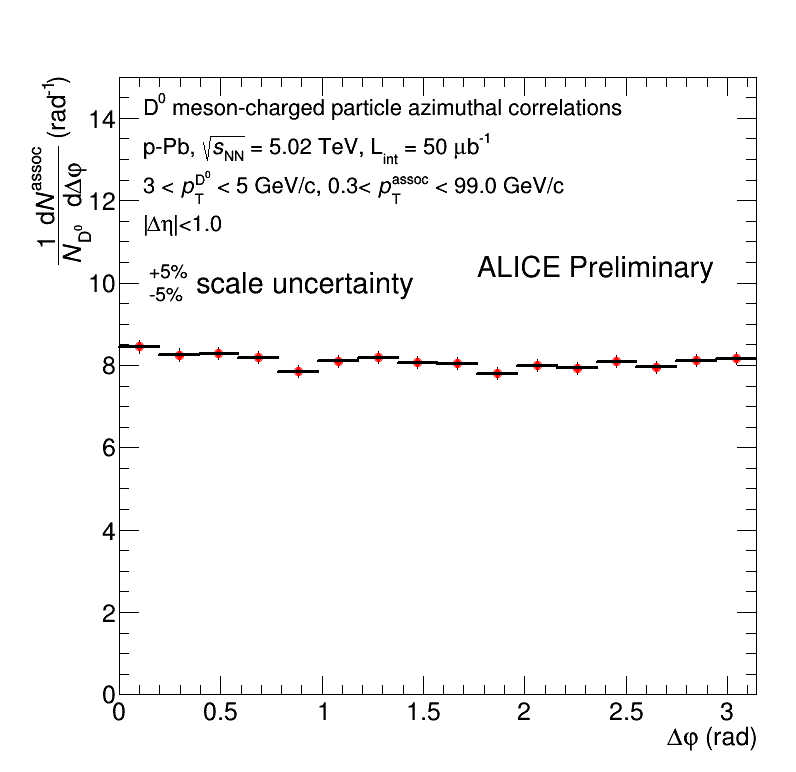
\includegraphics[width=0.32\linewidth]{figuresVsCent/Dzero/Correlations/020/CanvaAndVariedHistopPbDzeroPt3to5assocPt03to99.png}}
{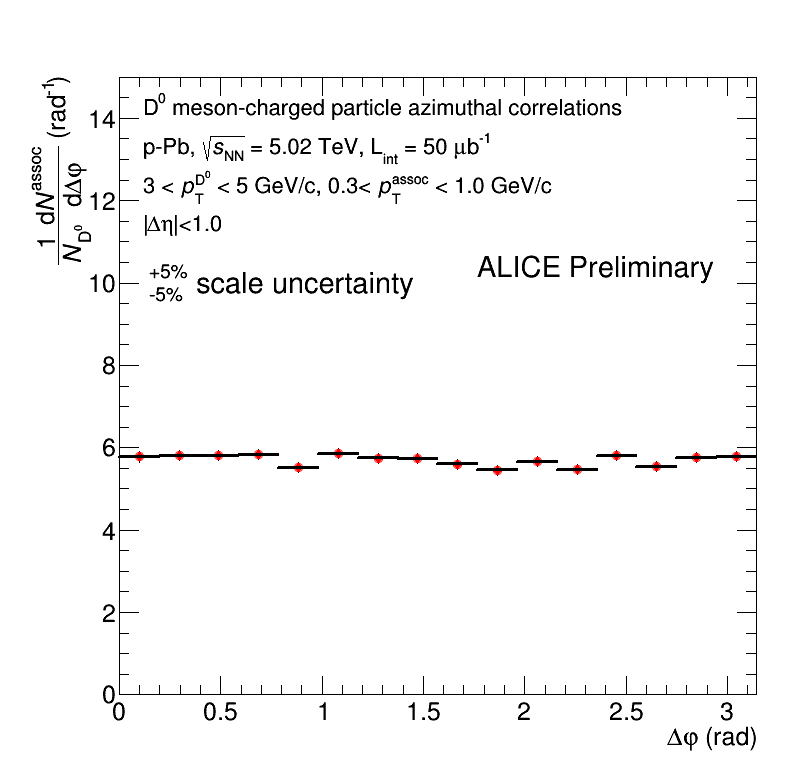
\includegraphics[width=0.32\linewidth]{figuresVsCent/Dzero/Correlations/020/CanvaAndVariedHistopPbDzeroPt3to5assocPt03to1.png}}
{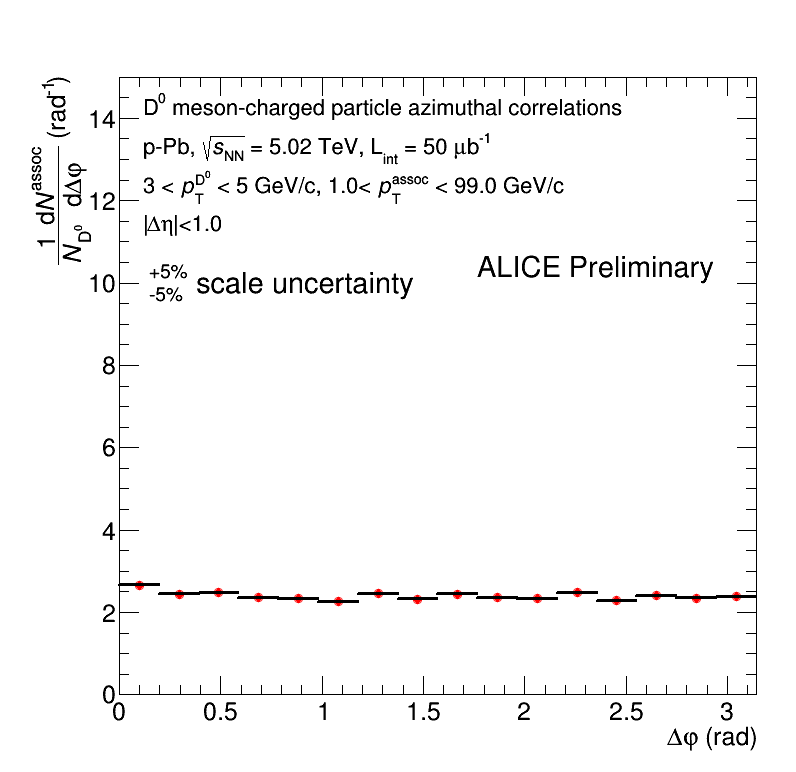
\includegraphics[width=0.32\linewidth]{figuresVsCent/Dzero/Correlations/020/CanvaAndVariedHistopPbDzeroPt3to5assocPt1to99.png}} \\
{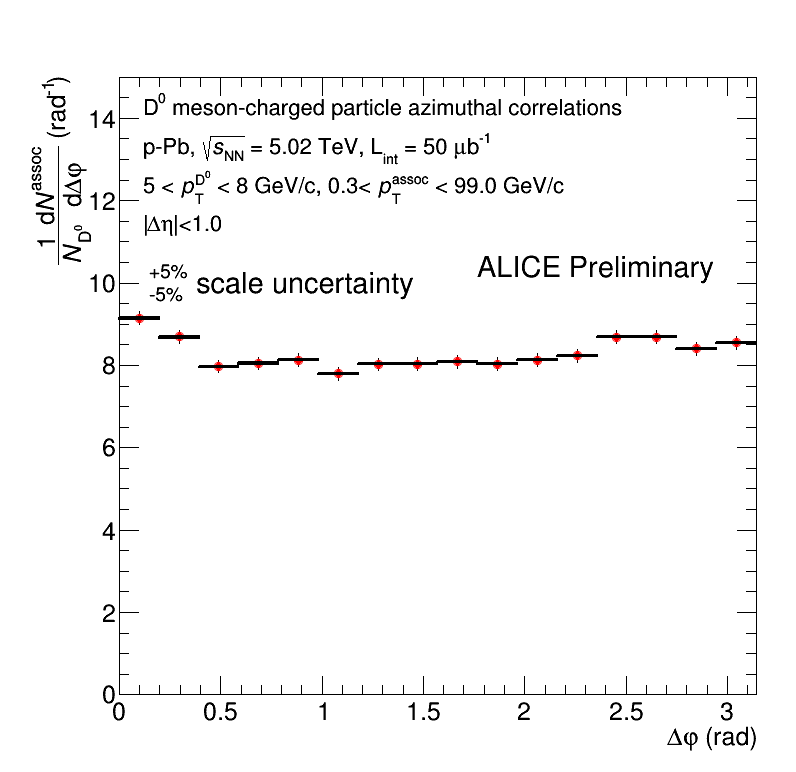
\includegraphics[width=0.32\linewidth]{figuresVsCent/Dzero/Correlations/020/CanvaAndVariedHistopPbDzeroPt5to8assocPt03to99.png}}
{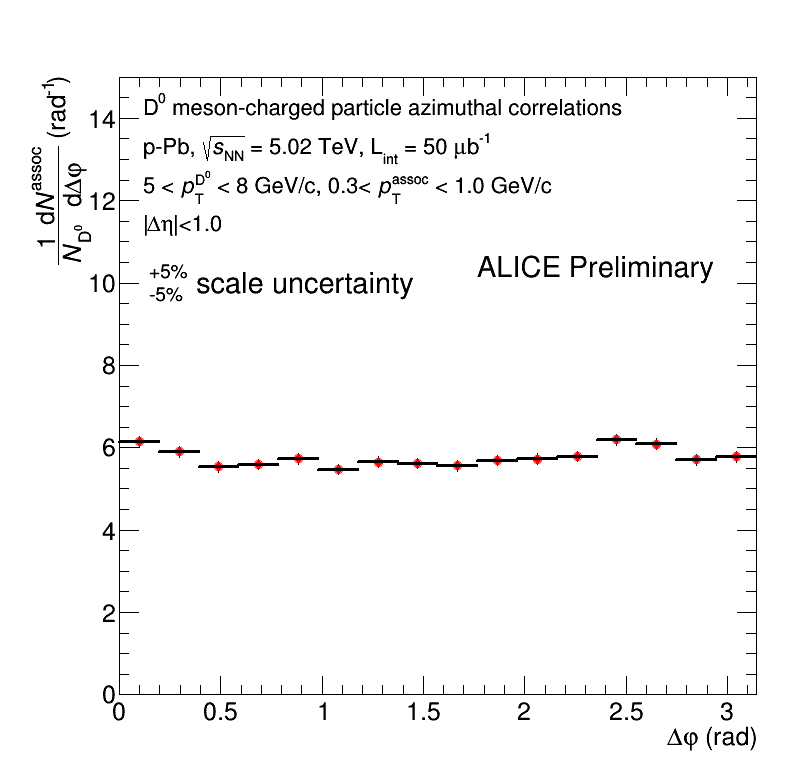
\includegraphics[width=0.32\linewidth]{figuresVsCent/Dzero/Correlations/020/CanvaAndVariedHistopPbDzeroPt5to8assocPt03to1.png}}
{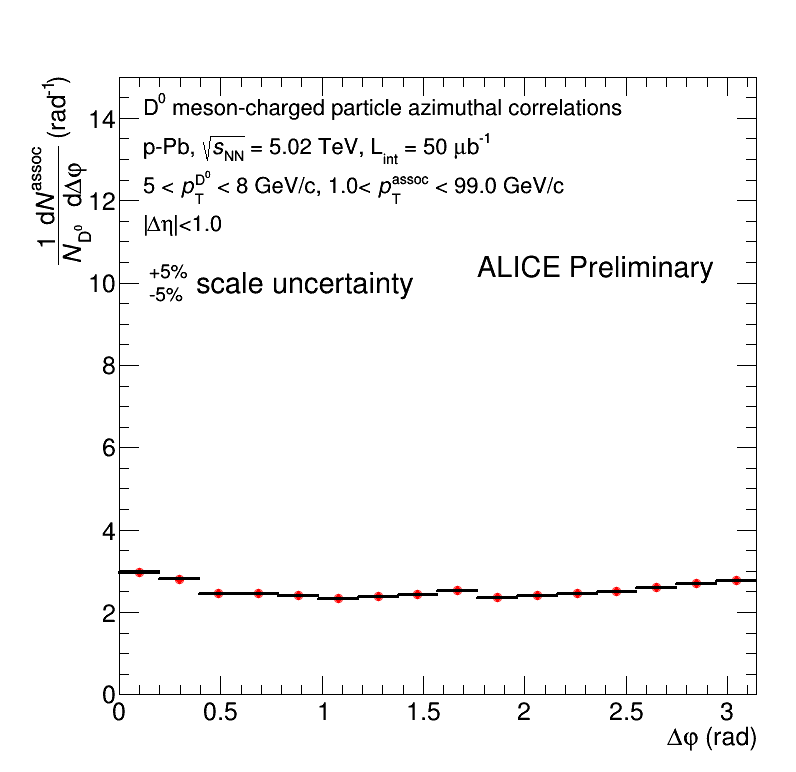
\includegraphics[width=0.32\linewidth]{figuresVsCent/Dzero/Correlations/020/CanvaAndVariedHistopPbDzeroPt5to8assocPt1to99.png}} \\
{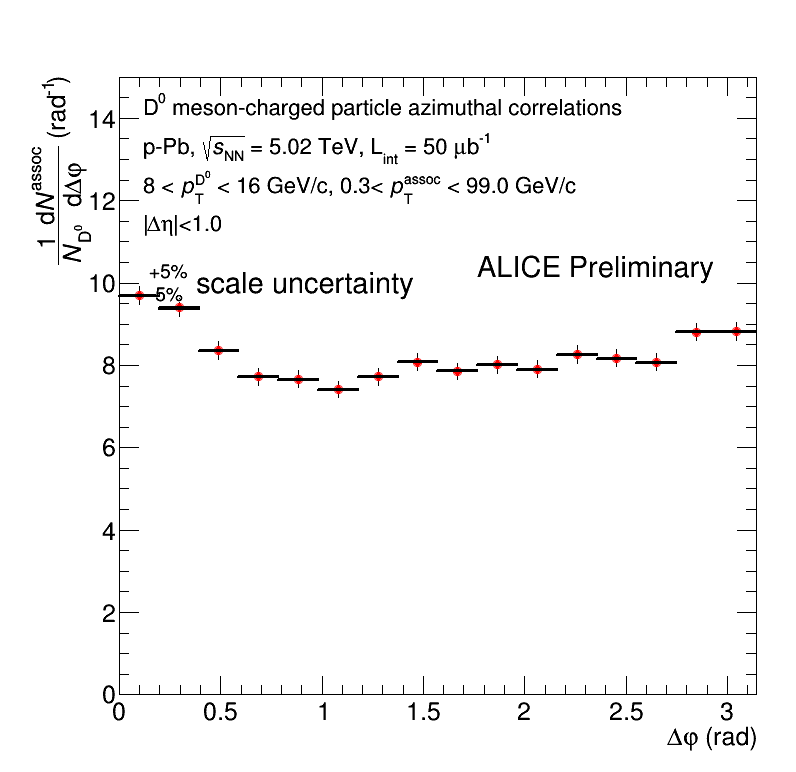
\includegraphics[width=0.32\linewidth]{figuresVsCent/Dzero/Correlations/020/CanvaAndVariedHistopPbDzeroPt8to16assocPt03to99.png}}
{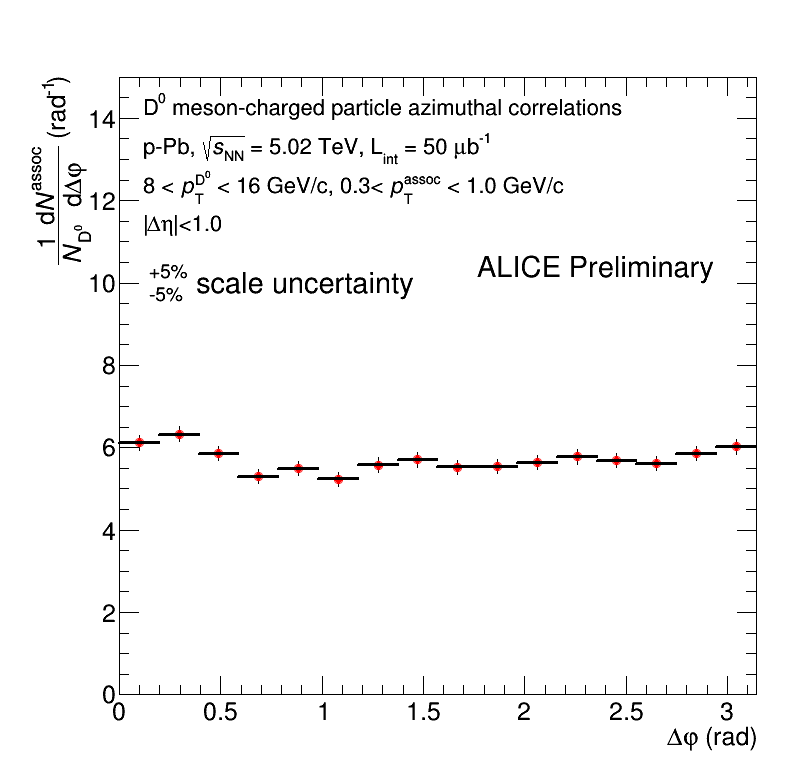
\includegraphics[width=0.32\linewidth]{figuresVsCent/Dzero/Correlations/020/CanvaAndVariedHistopPbDzeroPt8to16assocPt03to1.png}}
{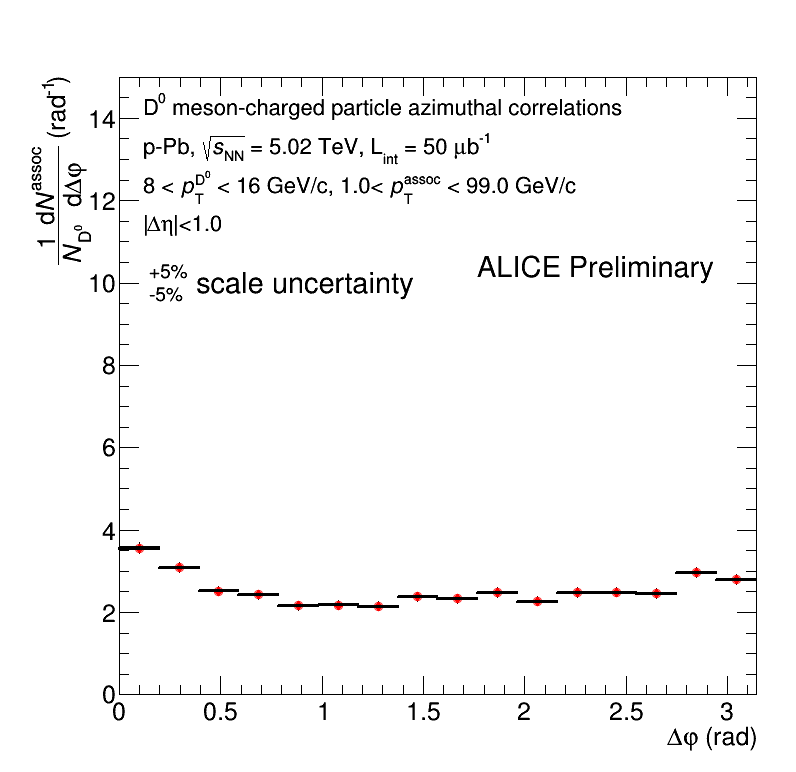
\includegraphics[width=0.32\linewidth]{figuresVsCent/Dzero/Correlations/020/CanvaAndVariedHistopPbDzeroPt8to16assocPt1to99.png}} \\
{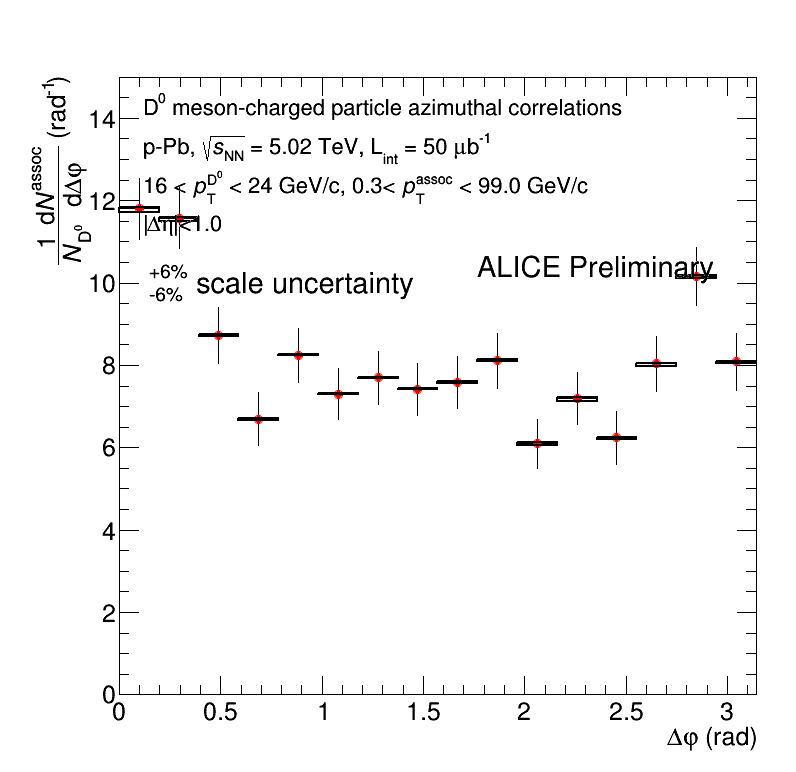
\includegraphics[width=0.32\linewidth]{figuresVsCent/Dzero/Correlations/020/CanvaAndVariedHistopPbDzeroPt16to24assocPt03to99.png}}
{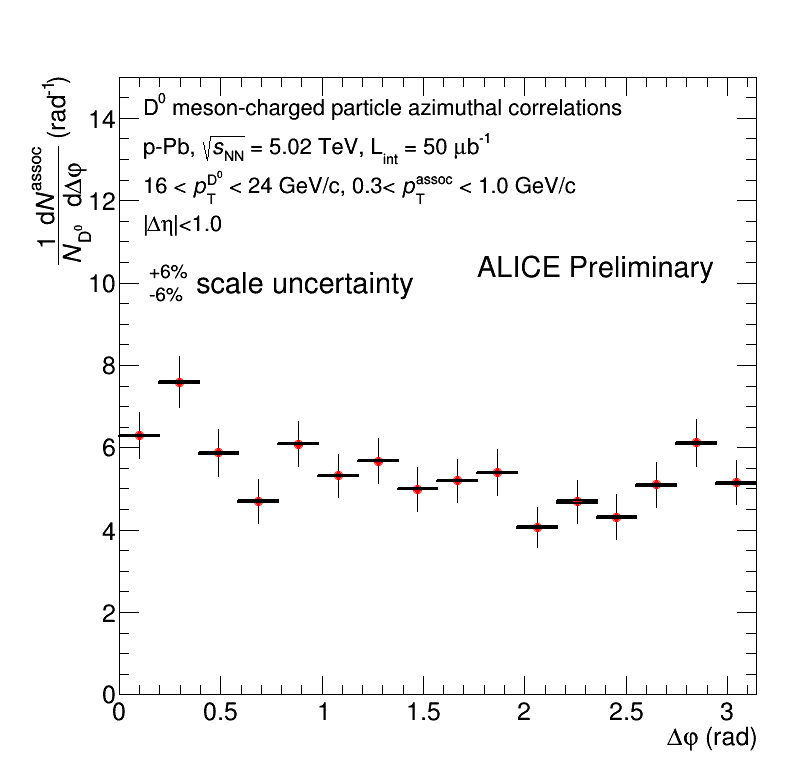
\includegraphics[width=0.32\linewidth]{figuresVsCent/Dzero/Correlations/020/CanvaAndVariedHistopPbDzeroPt16to24assocPt03to1.png}}
{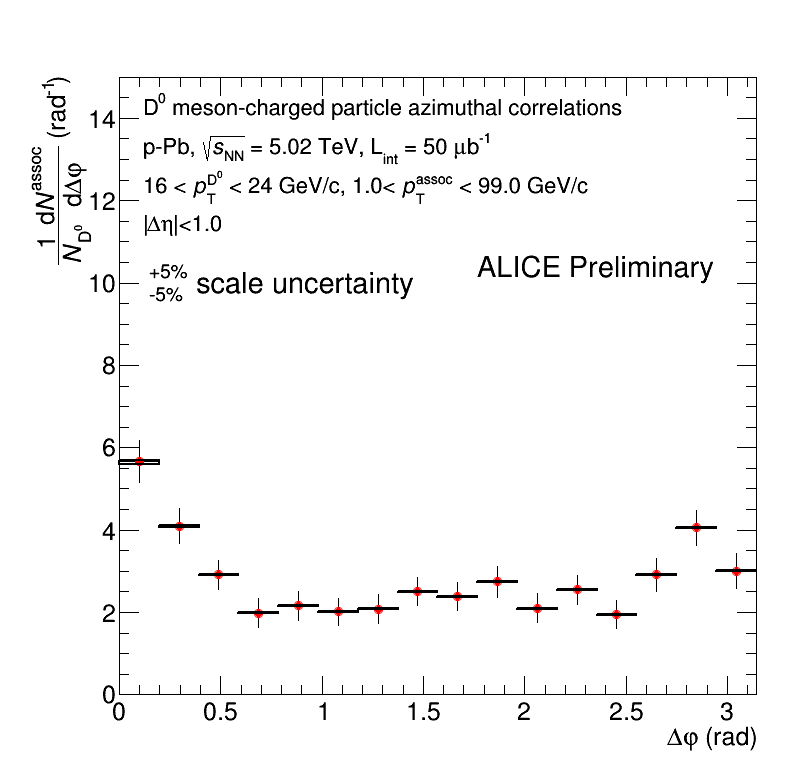
\includegraphics[width=0.32\linewidth]{figuresVsCent/Dzero/Correlations/020/CanvaAndVariedHistopPbDzeroPt16to24assocPt1to99.png}}
 \caption{Correlation distributions for $\Dzero$ meson as trigger particle (0-20\%). Each row is a different $\pt$(D) range, each column a different $\pt$(assoc) range. The systematic uncertainties labelled in the plots are not final. Note: the L=50 $\mu$b$^-1$ is a typo of the drawing macro (it shall be 300 $\mu$b$^-1$).}
\label{fig:Dzerocorr020}
\end{figure}

\begin{figure}
\centering
{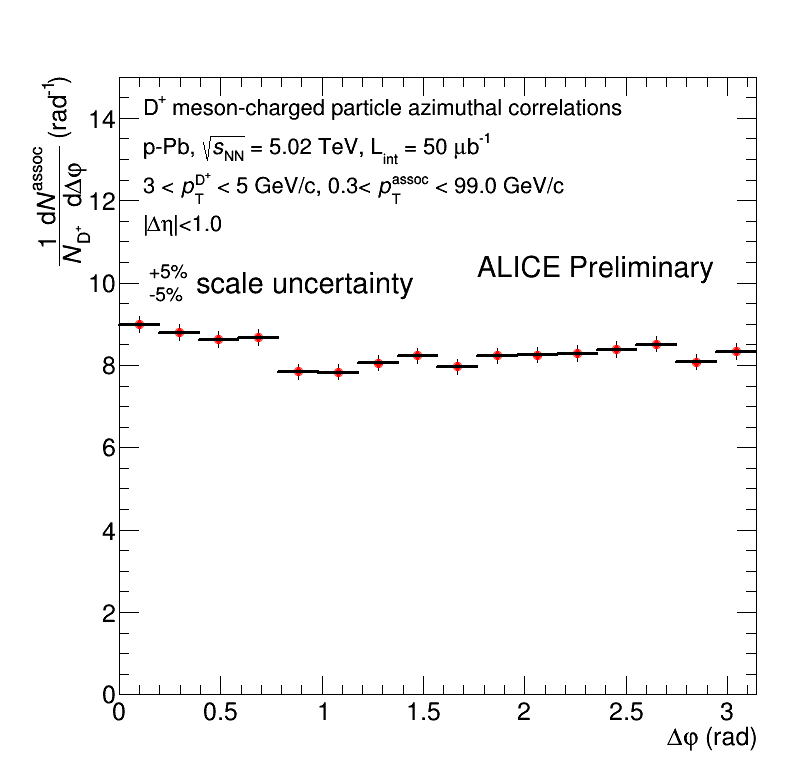
\includegraphics[width=0.32\linewidth]{figuresVsCent/Dplus/Correlations/020/CanvaAndVariedHistopPbDplusPt3to5assocPt03to99.png}}
{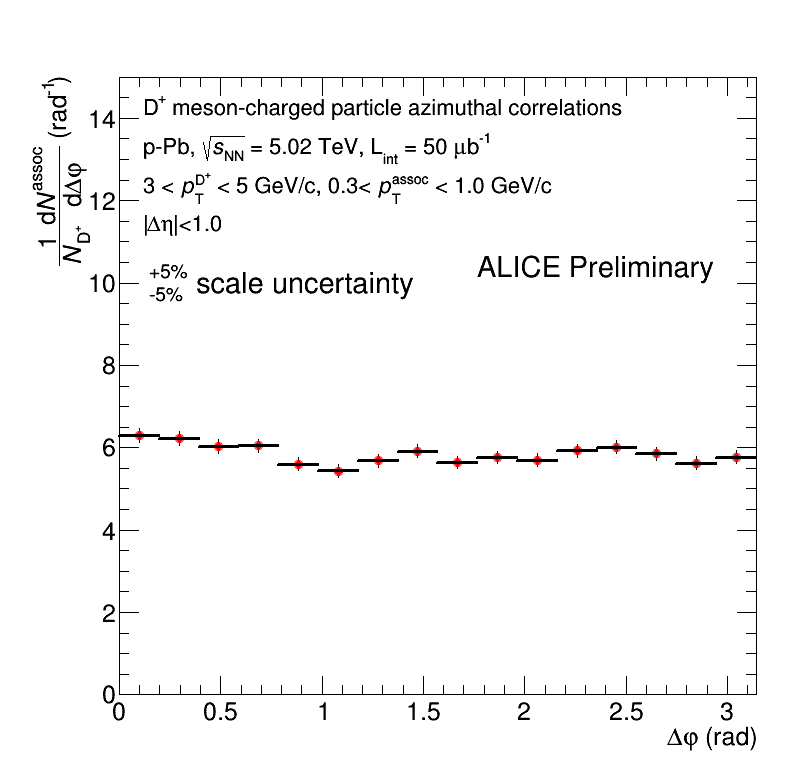
\includegraphics[width=0.32\linewidth]{figuresVsCent/Dplus/Correlations/020/CanvaAndVariedHistopPbDplusPt3to5assocPt03to1.png}}
{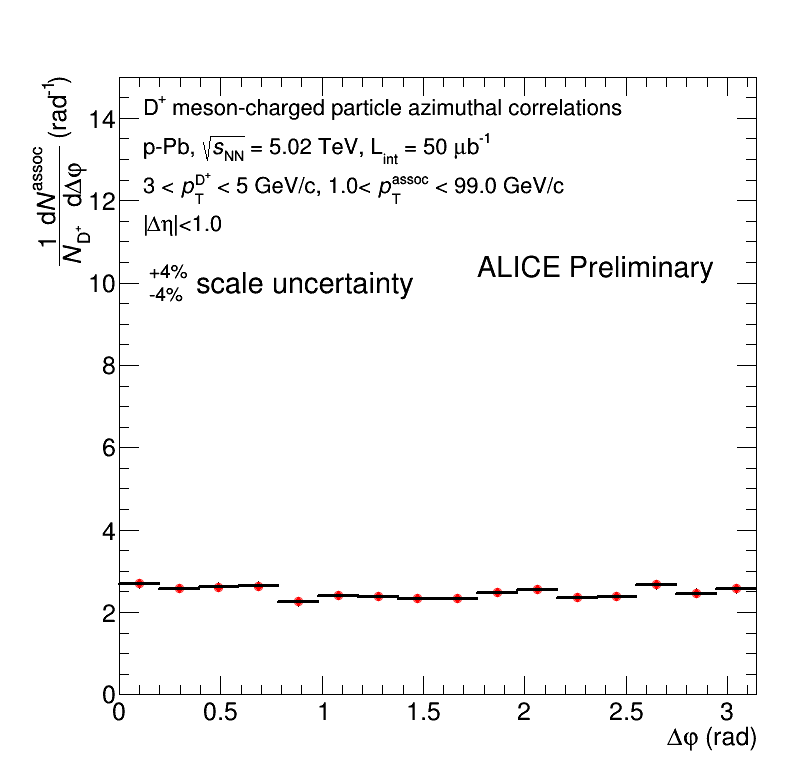
\includegraphics[width=0.32\linewidth]{figuresVsCent/Dplus/Correlations/020/CanvaAndVariedHistopPbDplusPt3to5assocPt1to99.png}} \\
{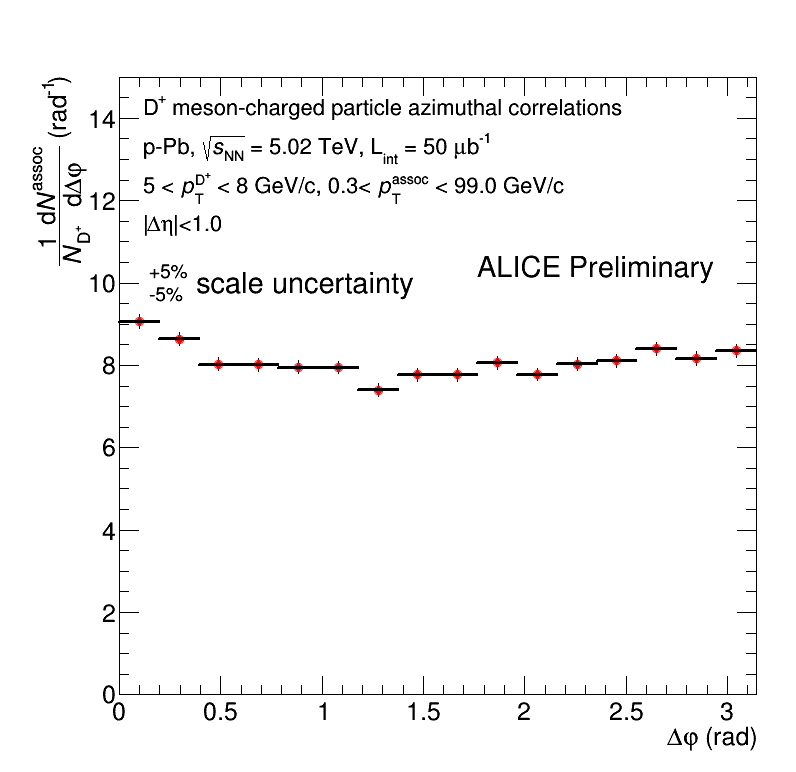
\includegraphics[width=0.32\linewidth]{figuresVsCent/Dplus/Correlations/020/CanvaAndVariedHistopPbDplusPt5to8assocPt03to99.png}}
{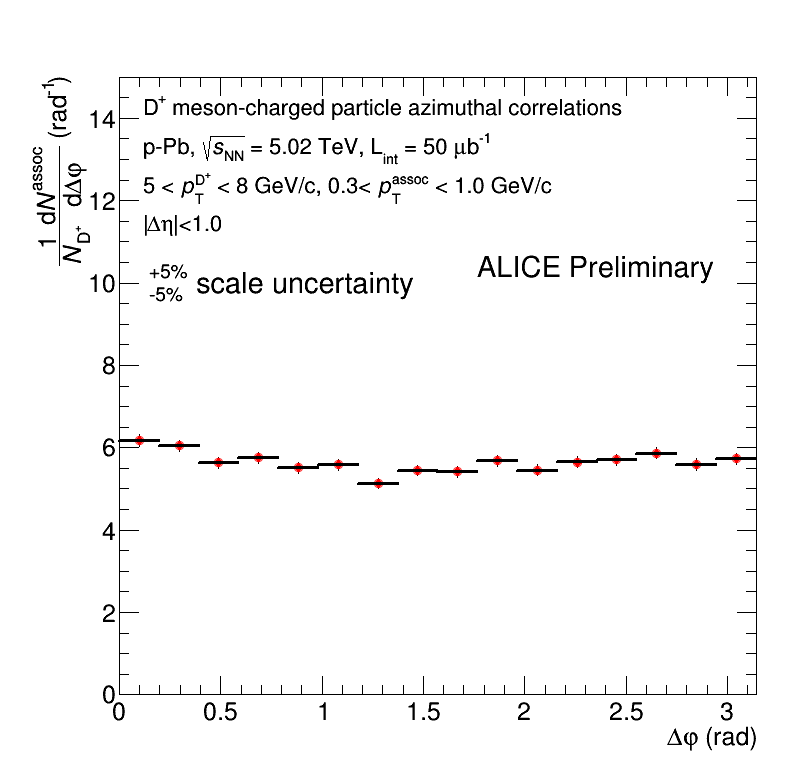
\includegraphics[width=0.32\linewidth]{figuresVsCent/Dplus/Correlations/020/CanvaAndVariedHistopPbDplusPt5to8assocPt03to1.png}}
{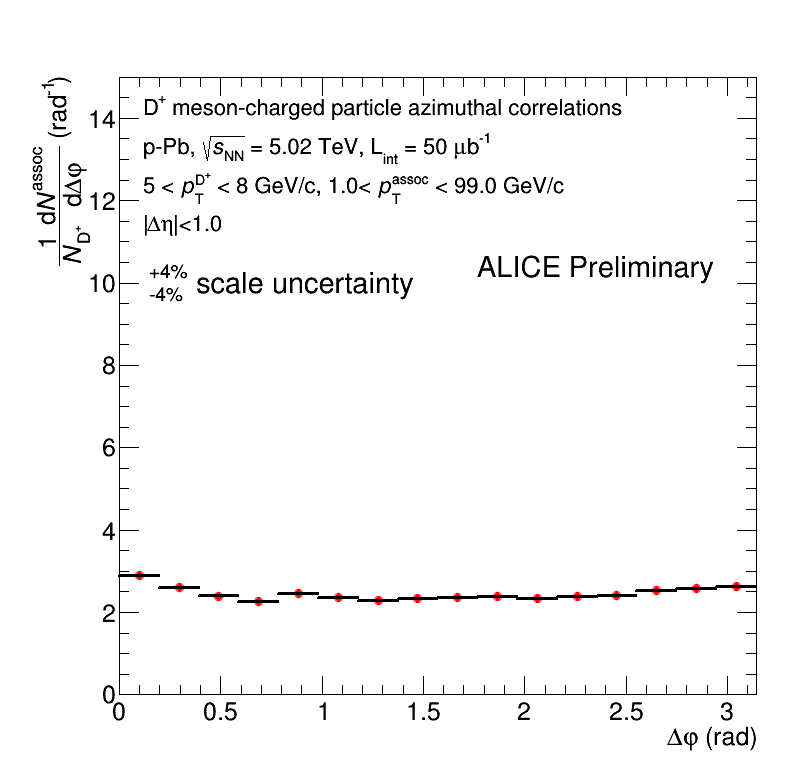
\includegraphics[width=0.32\linewidth]{figuresVsCent/Dplus/Correlations/020/CanvaAndVariedHistopPbDplusPt5to8assocPt1to99.png}} \\
{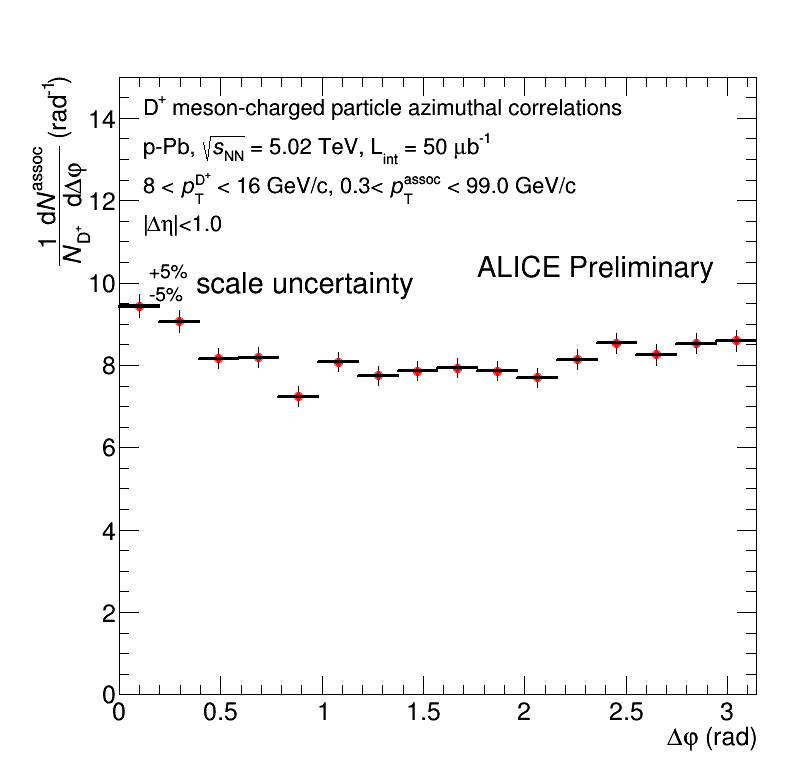
\includegraphics[width=0.32\linewidth]{figuresVsCent/Dplus/Correlations/020/CanvaAndVariedHistopPbDplusPt8to16assocPt03to99.png}}
{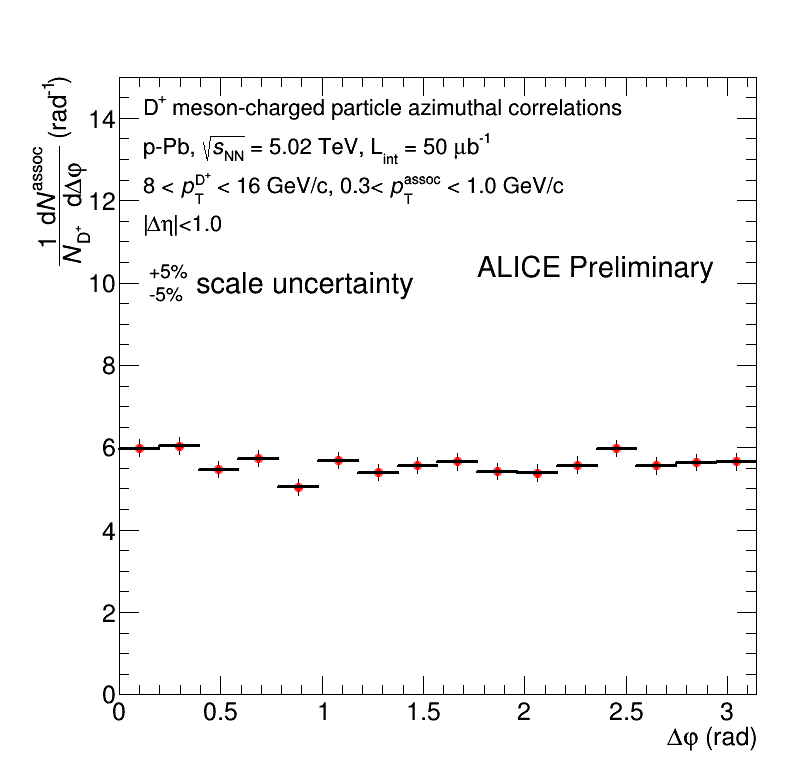
\includegraphics[width=0.32\linewidth]{figuresVsCent/Dplus/Correlations/020/CanvaAndVariedHistopPbDplusPt8to16assocPt03to1.png}}
{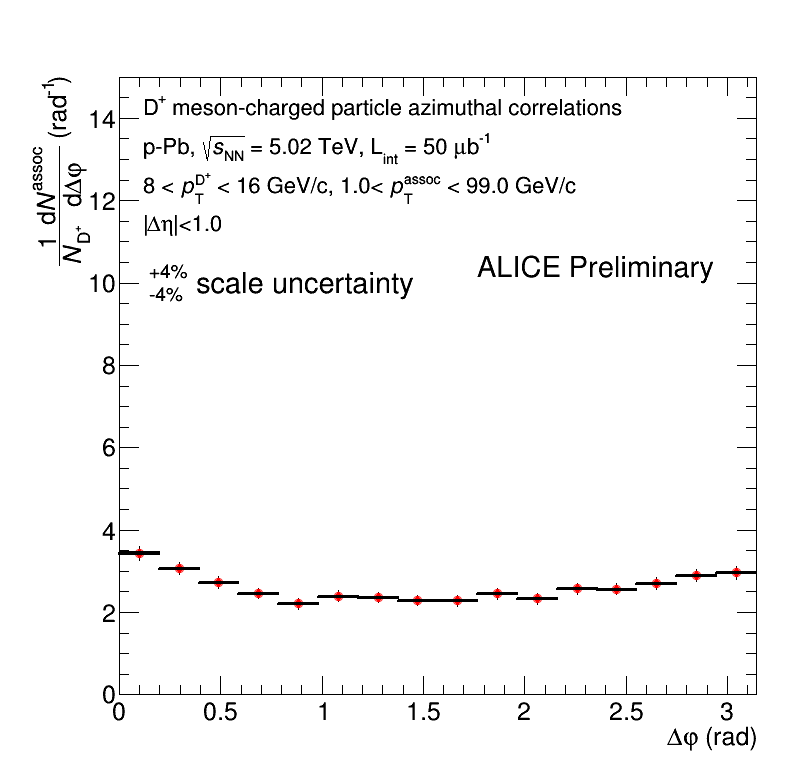
\includegraphics[width=0.32\linewidth]{figuresVsCent/Dplus/Correlations/020/CanvaAndVariedHistopPbDplusPt8to16assocPt1to99.png}} \\
{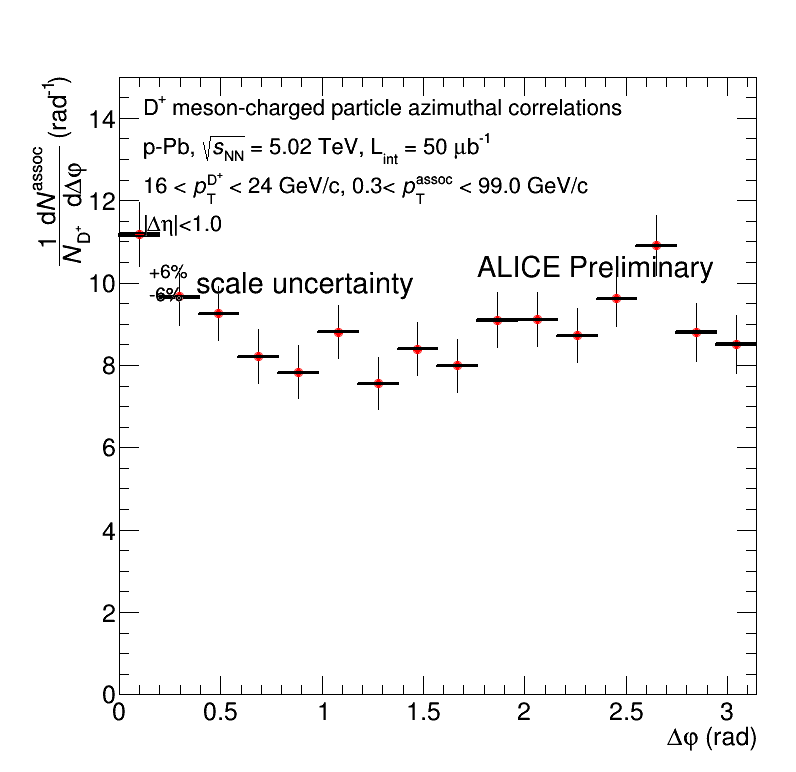
\includegraphics[width=0.32\linewidth]{figuresVsCent/Dplus/Correlations/020/CanvaAndVariedHistopPbDplusPt16to24assocPt03to99.png}}
{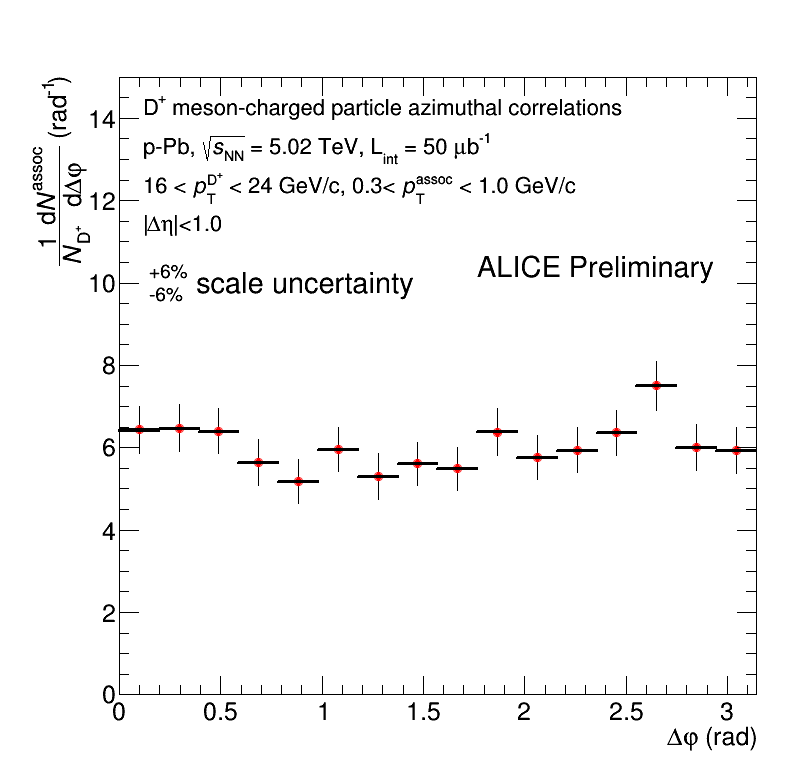
\includegraphics[width=0.32\linewidth]{figuresVsCent/Dplus/Correlations/020/CanvaAndVariedHistopPbDplusPt16to24assocPt03to1.png}}
{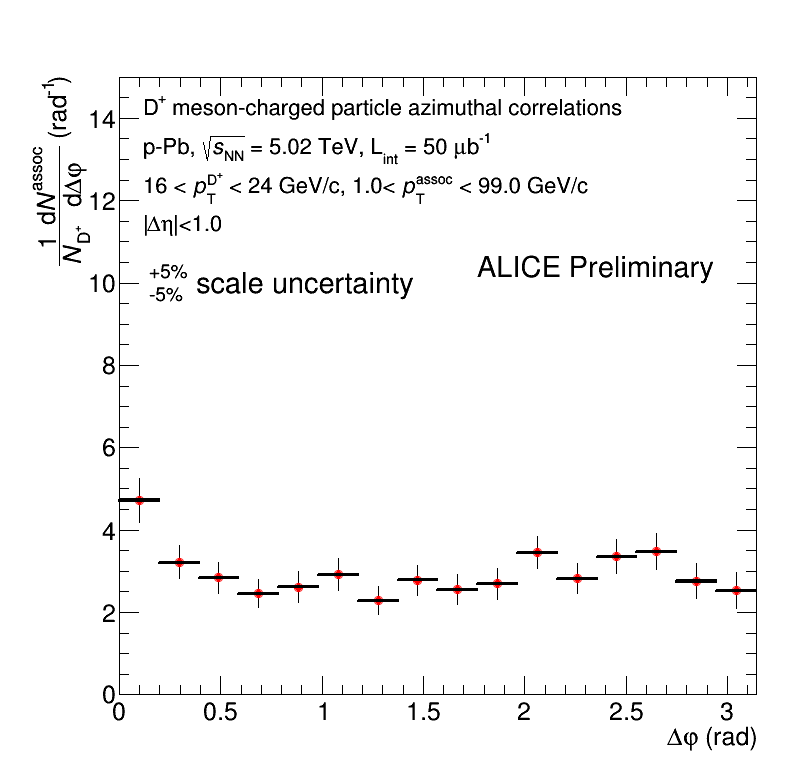
\includegraphics[width=0.32\linewidth]{figuresVsCent/Dplus/Correlations/020/CanvaAndVariedHistopPbDplusPt16to24assocPt1to99.png}}
 \caption{Correlation distributions for $\Dplus$ meson as trigger particle (0-20\%). Each row is a different $\pt$(D) range, each column a different $\pt$(assoc) range. The systematic uncertainties labelled in the plots are not final. Note: the L=50 $\mu$b$^-1$ is a typo of the drawing macro (it shall be 300 $\mu$b$^-1$).}
\label{fig:Dpluscorr020}
\end{figure}

\begin{figure}
\centering
{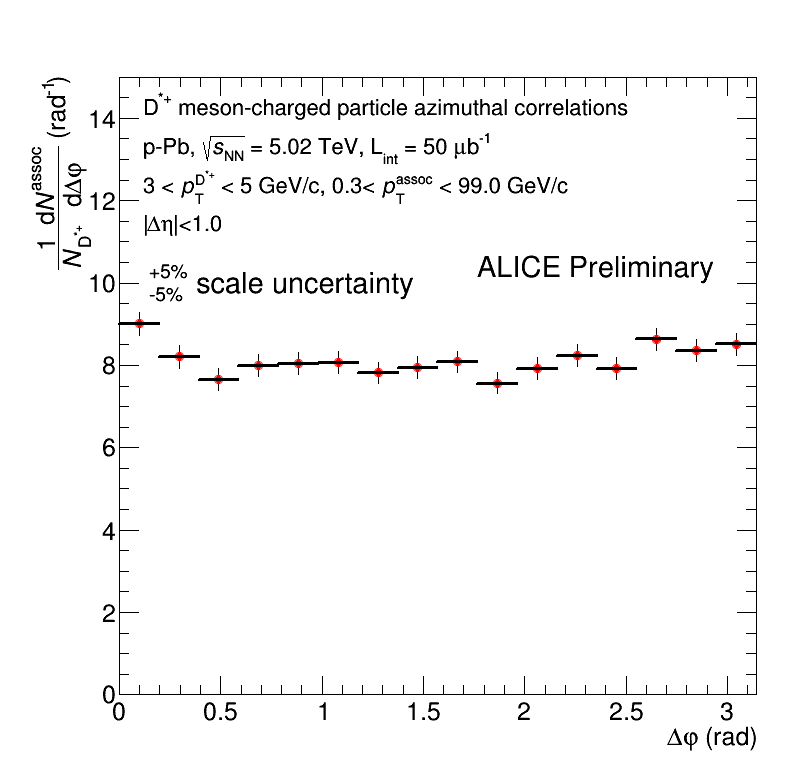
\includegraphics[width=0.32\linewidth]{figuresVsCent/Dstar/Correlations/020/CanvaAndVariedHistopPbDstarPt3to5assocPt03to99.png}}
{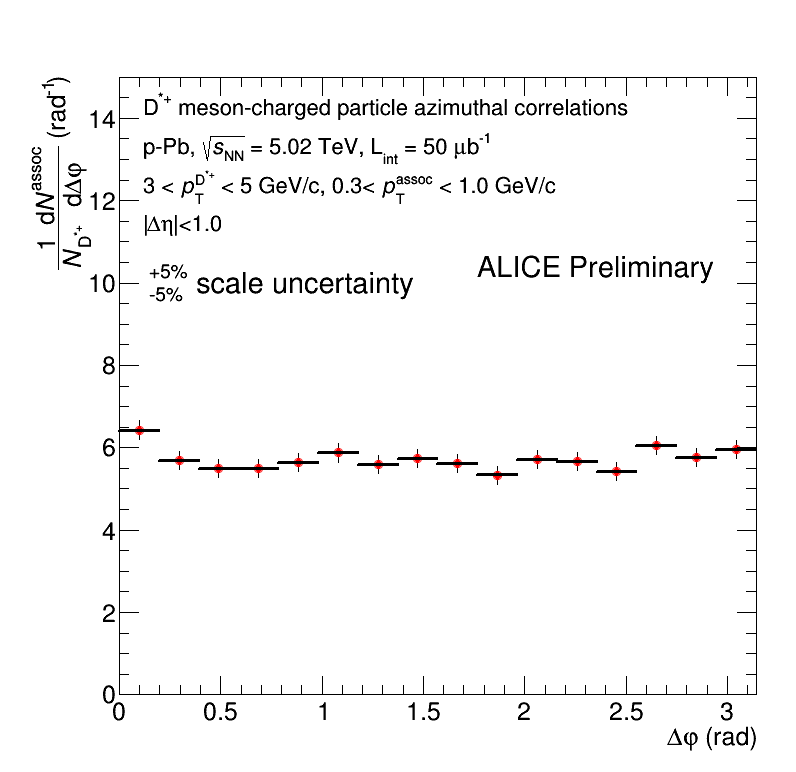
\includegraphics[width=0.32\linewidth]{figuresVsCent/Dstar/Correlations/020/CanvaAndVariedHistopPbDstarPt3to5assocPt03to1.png}}
{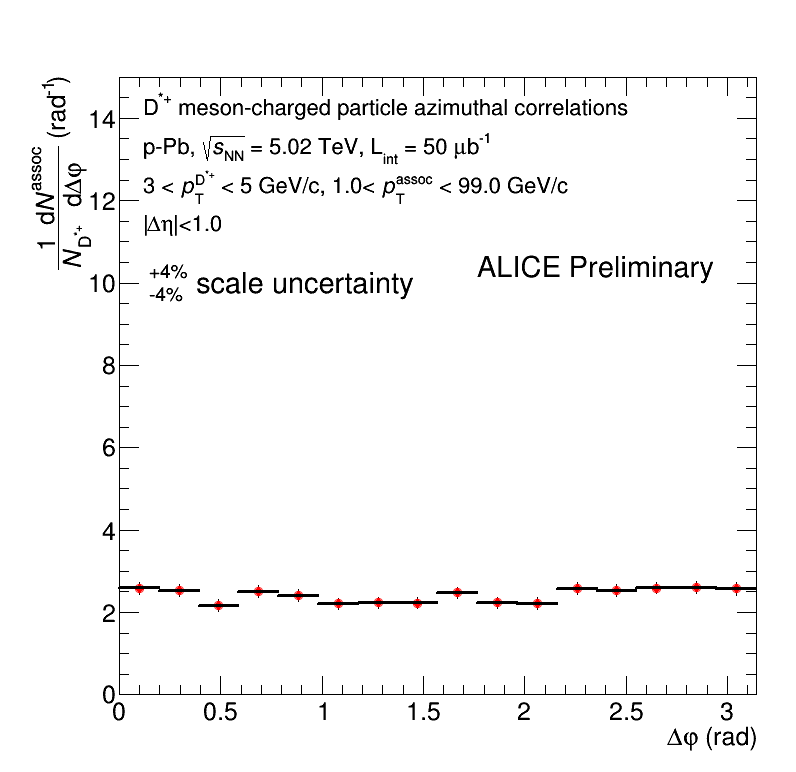
\includegraphics[width=0.32\linewidth]{figuresVsCent/Dstar/Correlations/020/CanvaAndVariedHistopPbDstarPt3to5assocPt1to99.png}} \\
{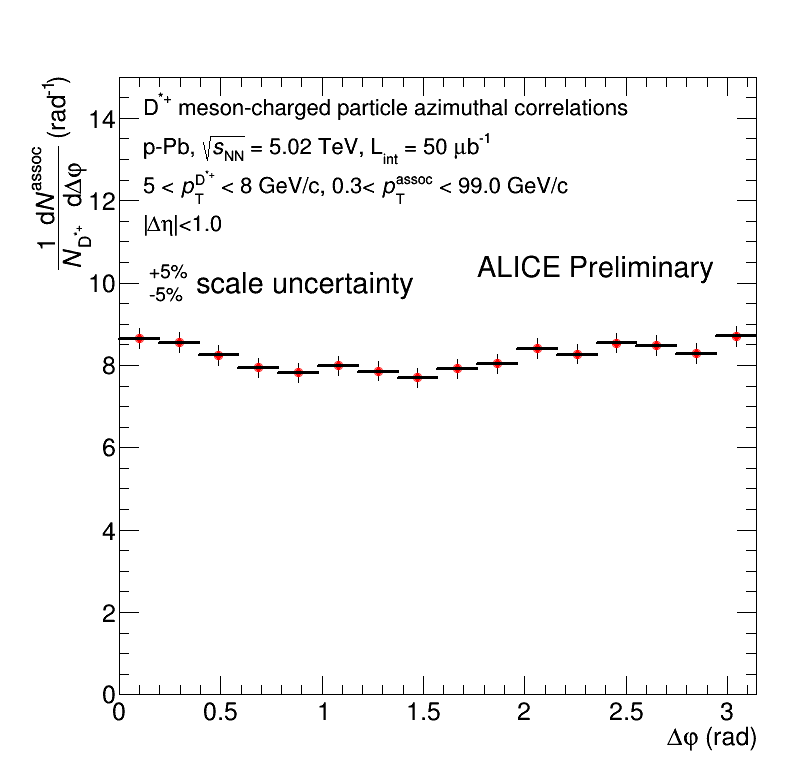
\includegraphics[width=0.32\linewidth]{figuresVsCent/Dstar/Correlations/020/CanvaAndVariedHistopPbDstarPt5to8assocPt03to99.png}}
{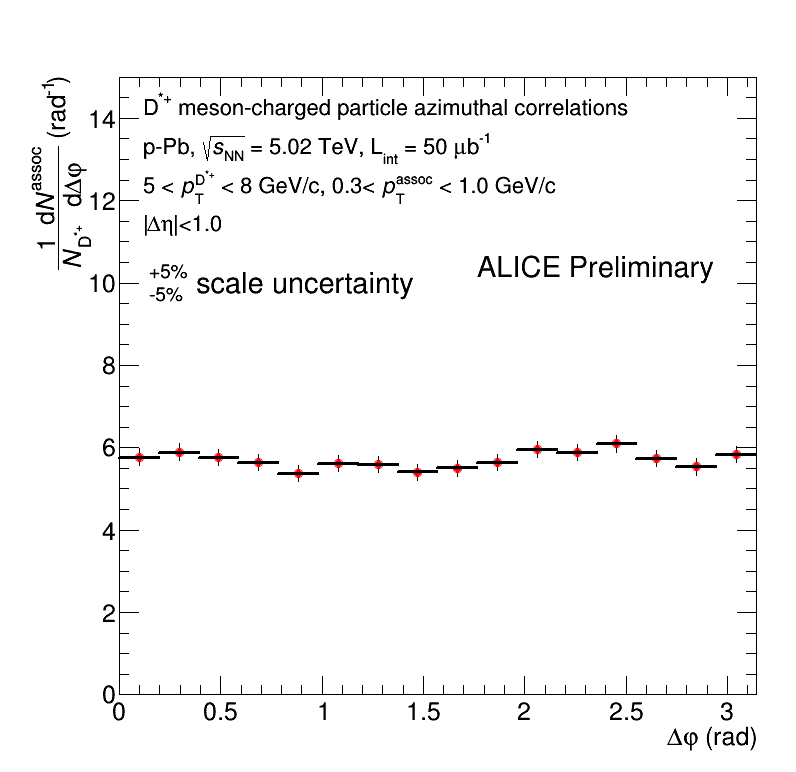
\includegraphics[width=0.32\linewidth]{figuresVsCent/Dstar/Correlations/020/CanvaAndVariedHistopPbDstarPt5to8assocPt03to1.png}}
{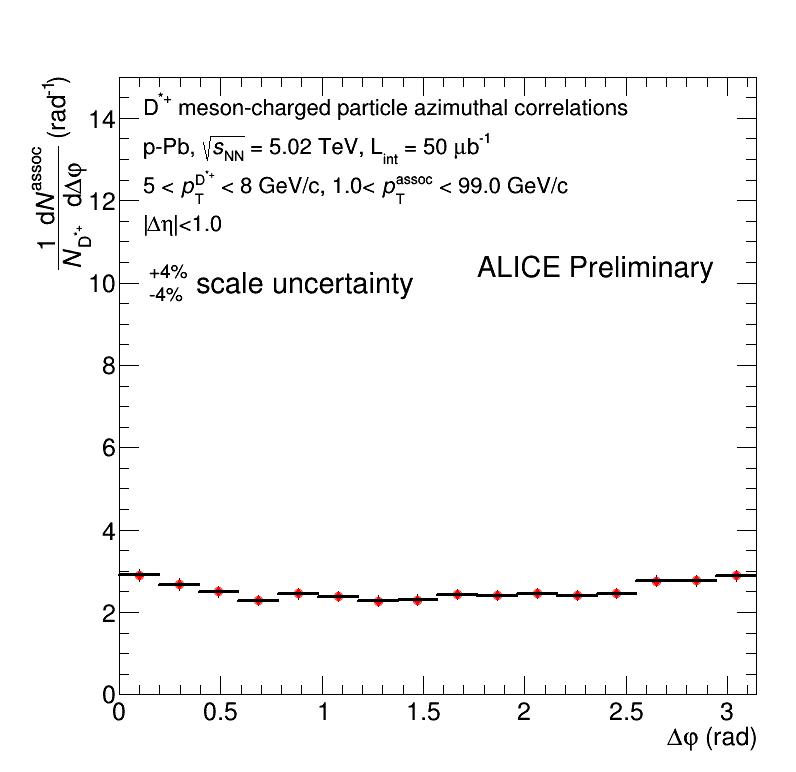
\includegraphics[width=0.32\linewidth]{figuresVsCent/Dstar/Correlations/020/CanvaAndVariedHistopPbDstarPt5to8assocPt1to99.png}} \\
{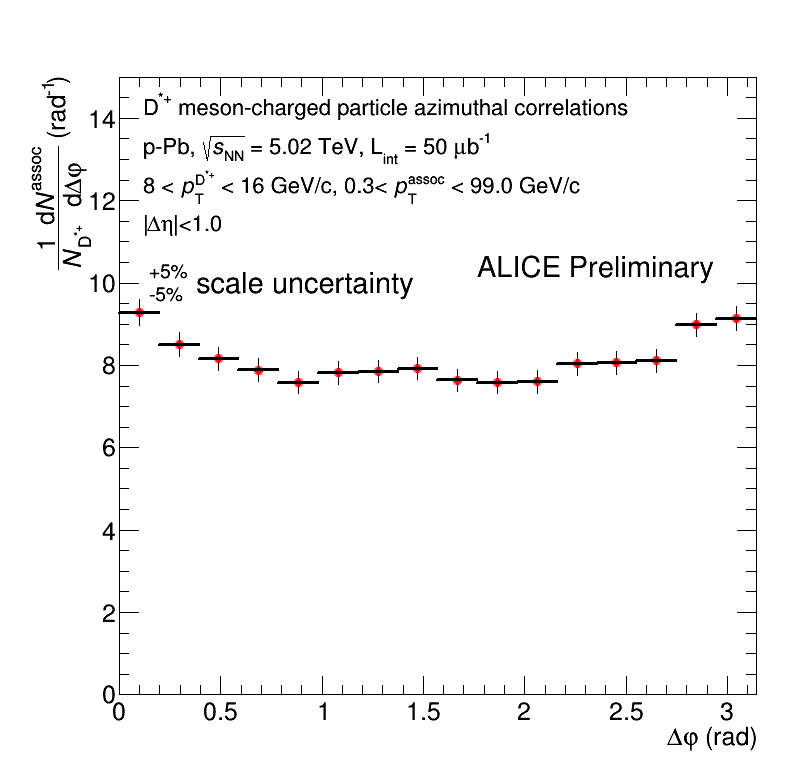
\includegraphics[width=0.32\linewidth]{figuresVsCent/Dstar/Correlations/020/CanvaAndVariedHistopPbDstarPt8to16assocPt03to99.png}}
{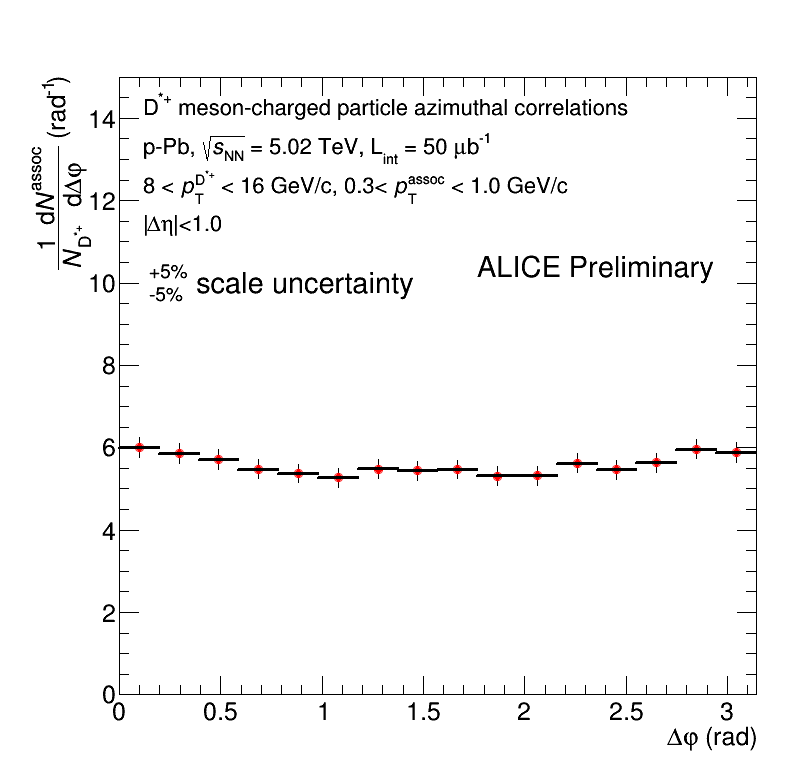
\includegraphics[width=0.32\linewidth]{figuresVsCent/Dstar/Correlations/020/CanvaAndVariedHistopPbDstarPt8to16assocPt03to1.png}}
{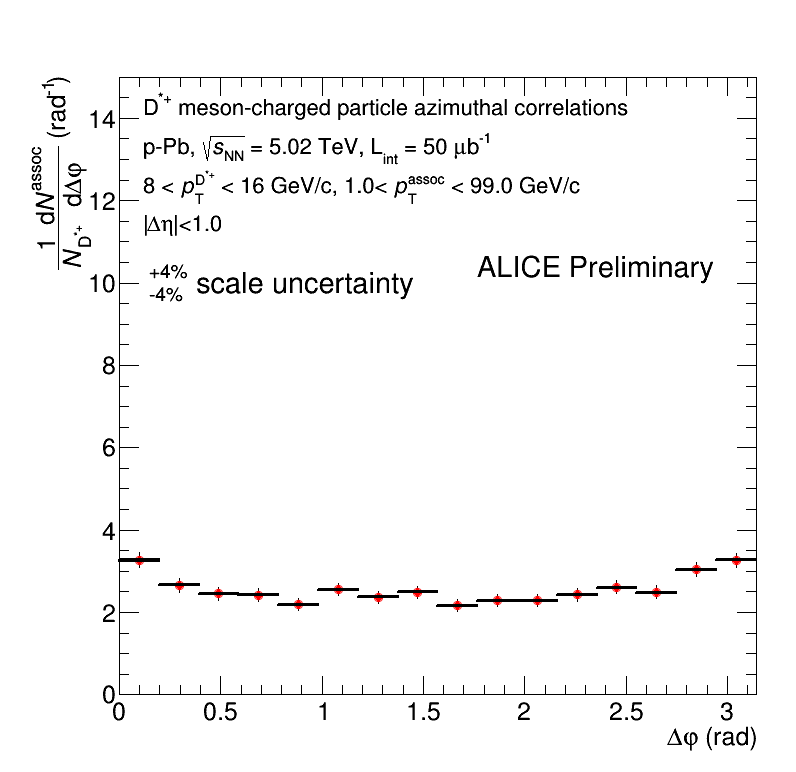
\includegraphics[width=0.32\linewidth]{figuresVsCent/Dstar/Correlations/020/CanvaAndVariedHistopPbDstarPt8to16assocPt1to99.png}} \\
{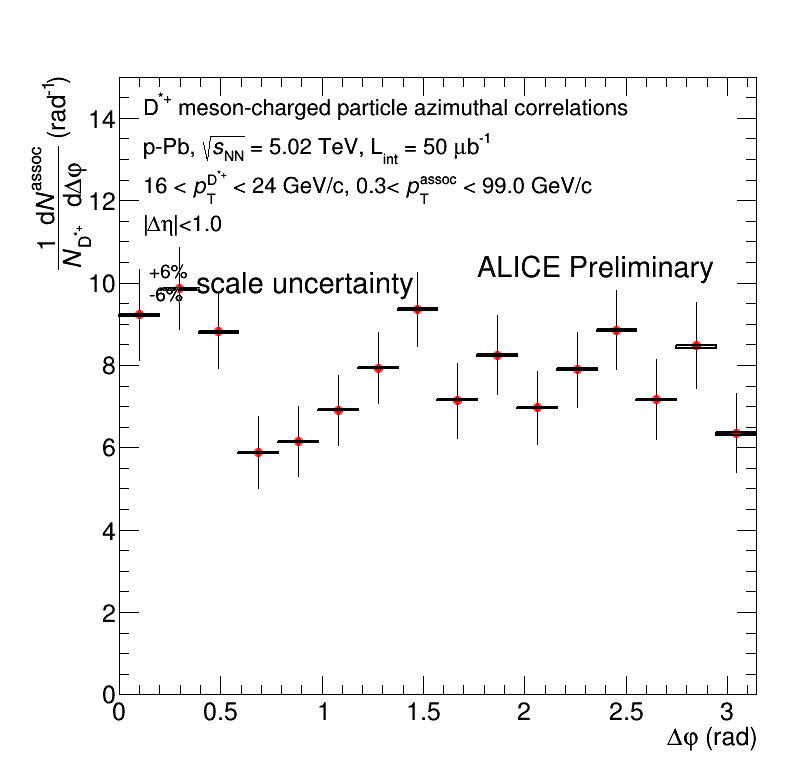
\includegraphics[width=0.32\linewidth]{figuresVsCent/Dstar/Correlations/020/CanvaAndVariedHistopPbDstarPt16to24assocPt03to99.png}}
{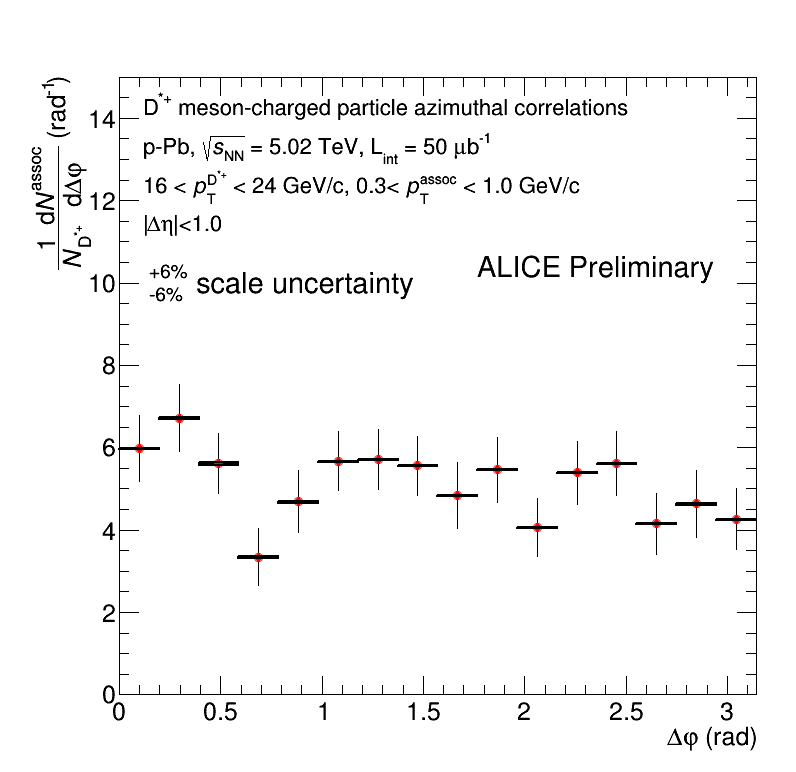
\includegraphics[width=0.32\linewidth]{figuresVsCent/Dstar/Correlations/020/CanvaAndVariedHistopPbDstarPt16to24assocPt03to1.png}}
{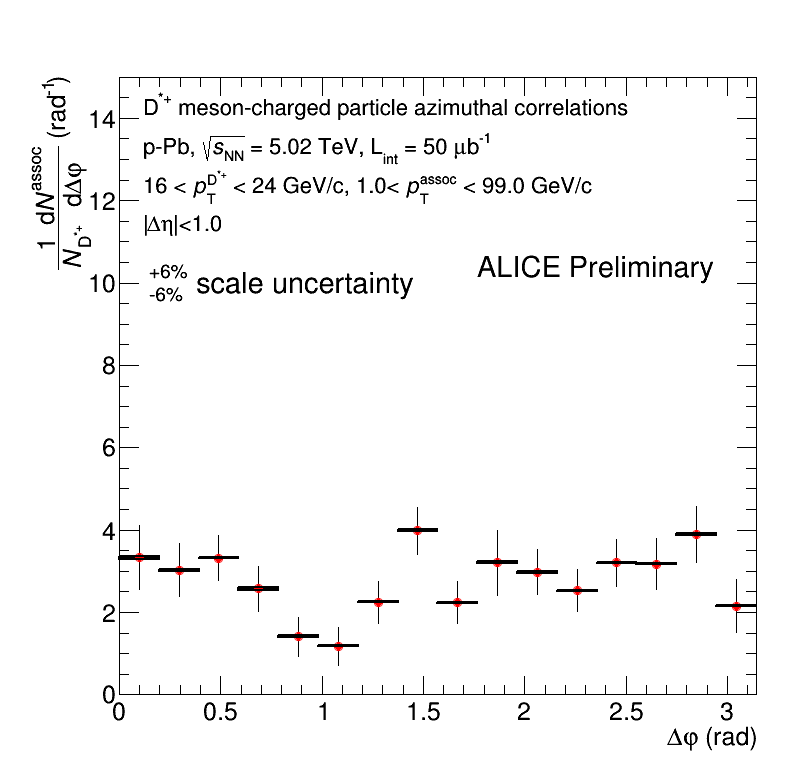
\includegraphics[width=0.32\linewidth]{figuresVsCent/Dstar/Correlations/020/CanvaAndVariedHistopPbDstarPt16to24assocPt1to99.png}}
 \caption{Correlation distributions for $\Dstar$ meson as trigger particle (0-20\%). Each row is a different $\pt$(D) range, each column a different $\pt$(assoc) range. The systematic uncertainties labelled in the plots are not final. Note: the L=50 $\mu$b$^-1$ is a typo of the drawing macro (it shall be 300 $\mu$b$^-1$).}
\label{fig:Dstarcorr020}
\end{figure}

\begin{figure}
\centering
{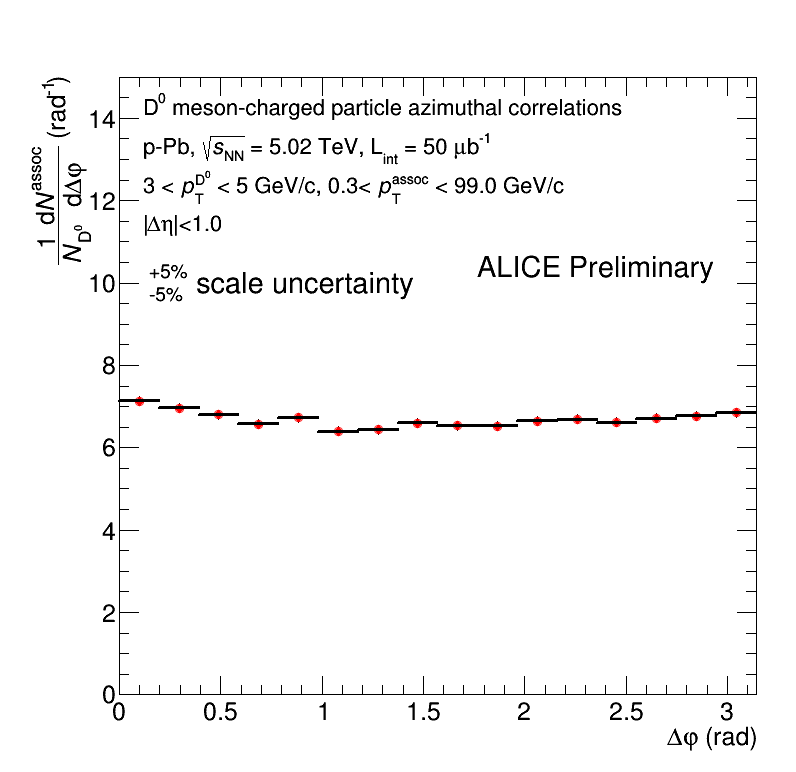
\includegraphics[width=0.32\linewidth]{figuresVsCent/Dzero/Correlations/2060/CanvaAndVariedHistopPbDzeroPt3to5assocPt03to99.png}}
{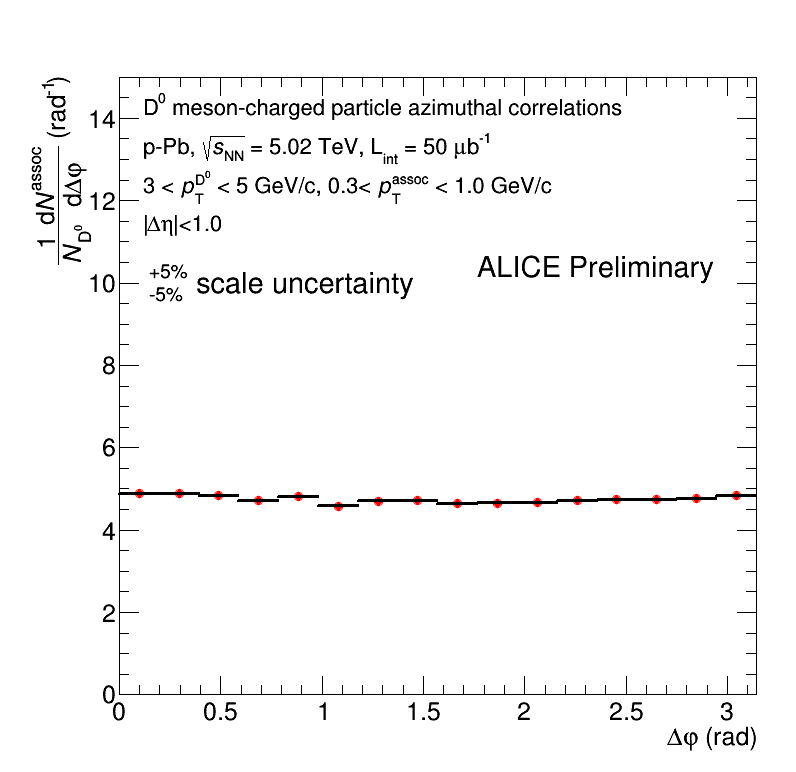
\includegraphics[width=0.32\linewidth]{figuresVsCent/Dzero/Correlations/2060/CanvaAndVariedHistopPbDzeroPt3to5assocPt03to1.png}}
{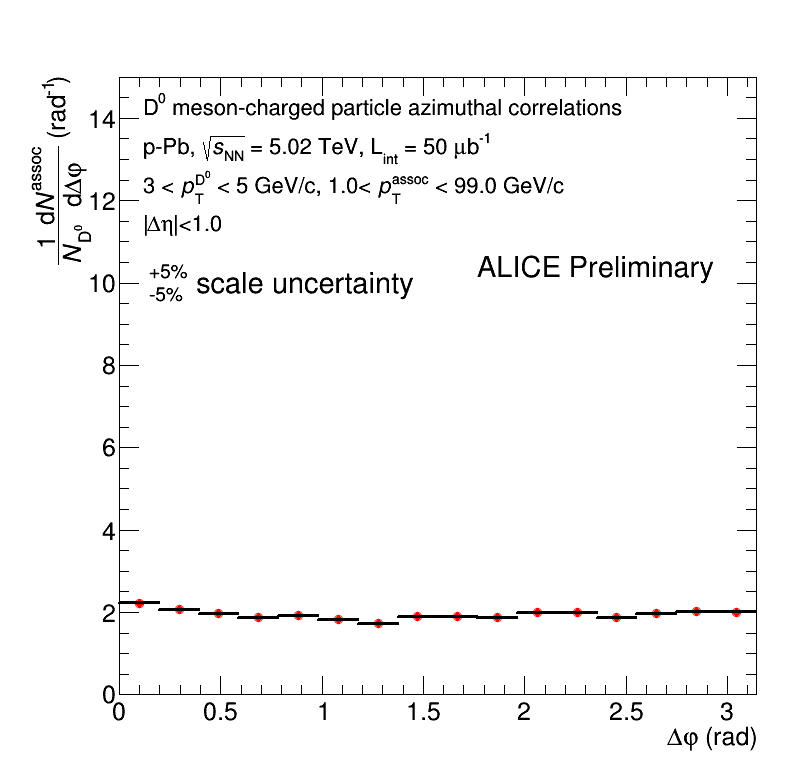
\includegraphics[width=0.32\linewidth]{figuresVsCent/Dzero/Correlations/2060/CanvaAndVariedHistopPbDzeroPt3to5assocPt1to99.png}} \\
{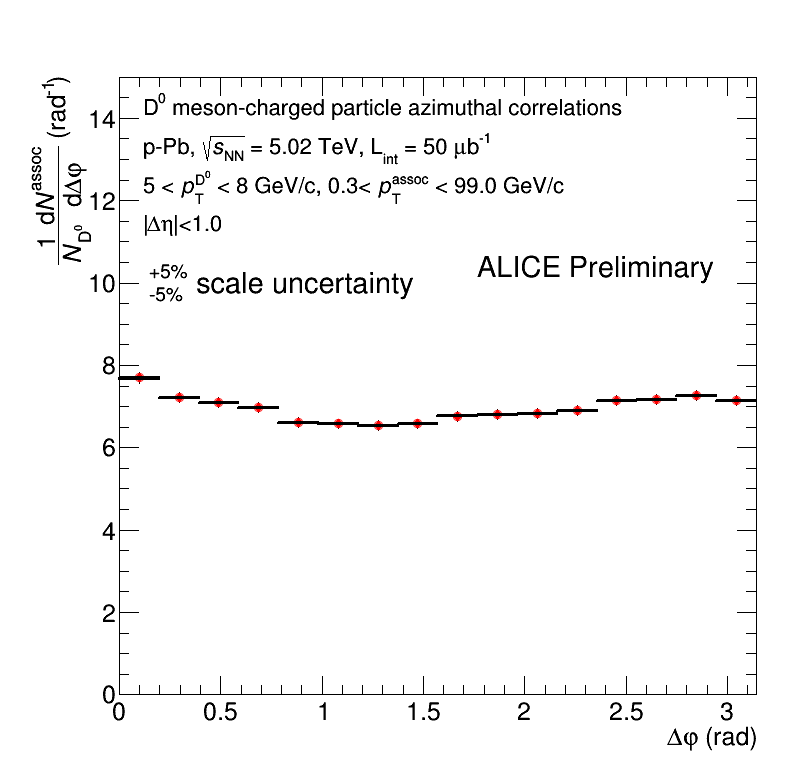
\includegraphics[width=0.32\linewidth]{figuresVsCent/Dzero/Correlations/2060/CanvaAndVariedHistopPbDzeroPt5to8assocPt03to99.png}}
{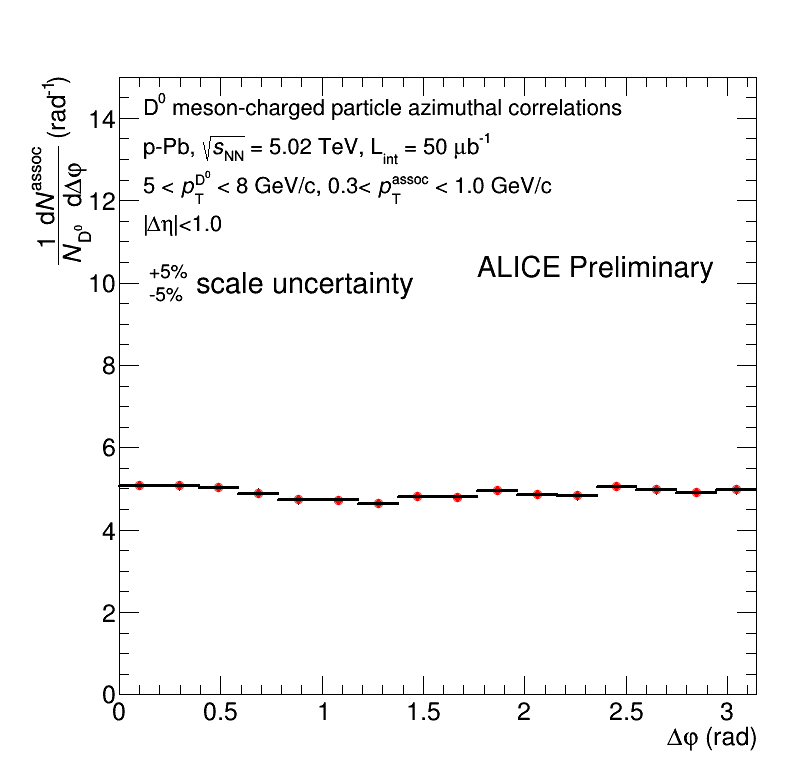
\includegraphics[width=0.32\linewidth]{figuresVsCent/Dzero/Correlations/2060/CanvaAndVariedHistopPbDzeroPt5to8assocPt03to1.png}}
{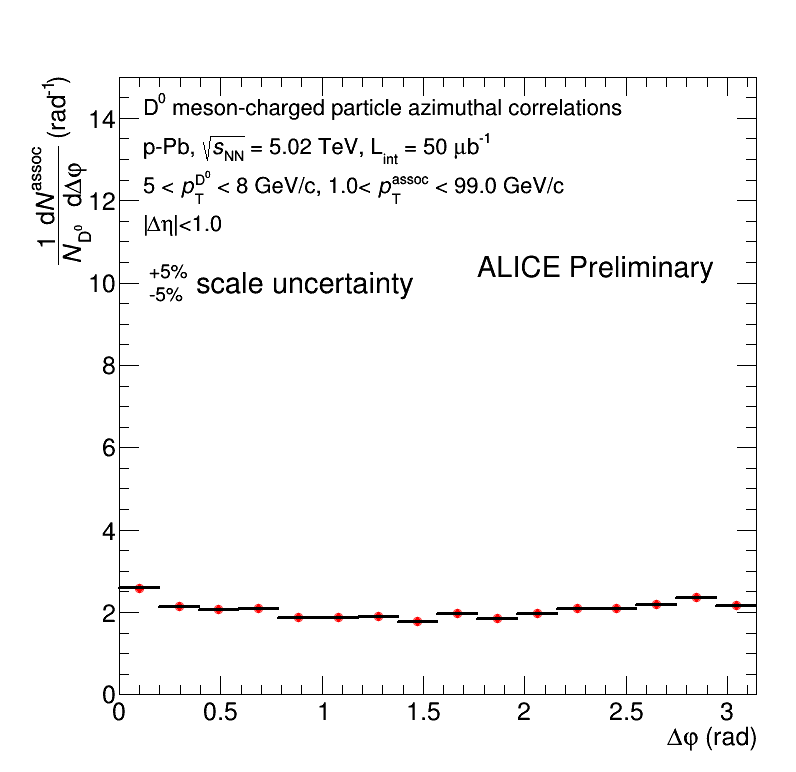
\includegraphics[width=0.32\linewidth]{figuresVsCent/Dzero/Correlations/2060/CanvaAndVariedHistopPbDzeroPt5to8assocPt1to99.png}} \\
{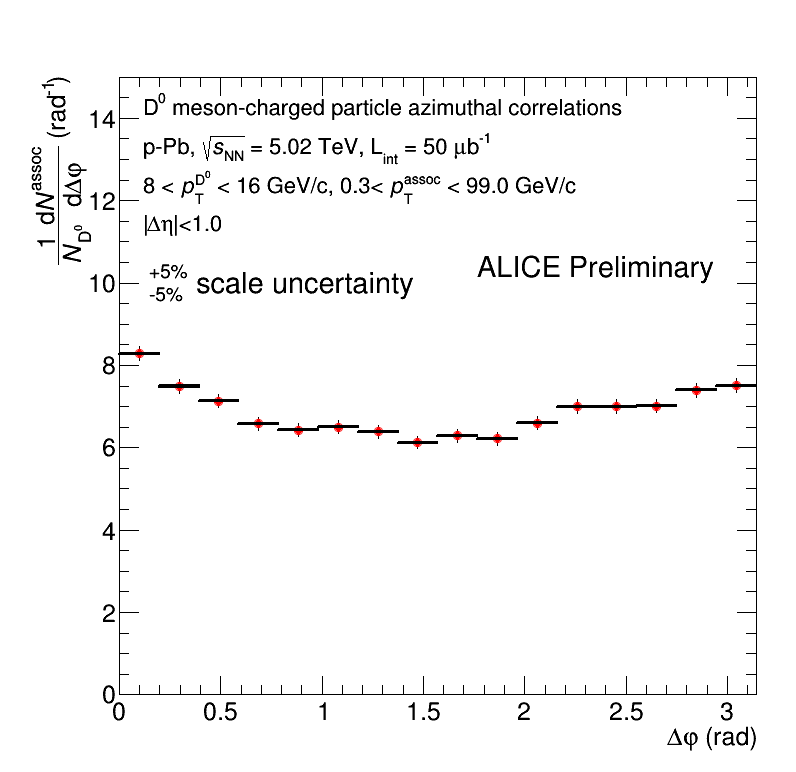
\includegraphics[width=0.32\linewidth]{figuresVsCent/Dzero/Correlations/2060/CanvaAndVariedHistopPbDzeroPt8to16assocPt03to99.png}}
{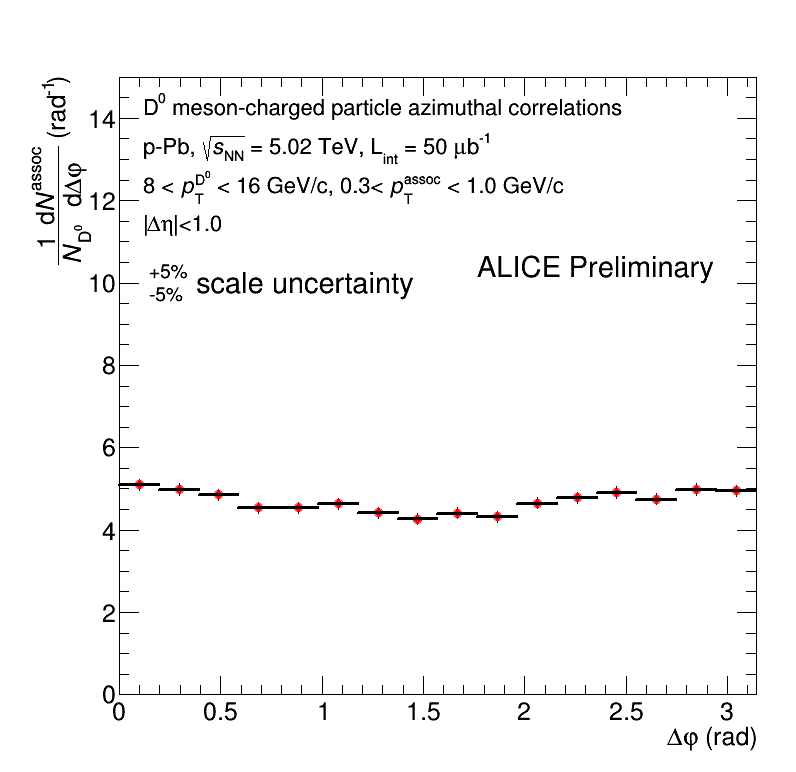
\includegraphics[width=0.32\linewidth]{figuresVsCent/Dzero/Correlations/2060/CanvaAndVariedHistopPbDzeroPt8to16assocPt03to1.png}}
{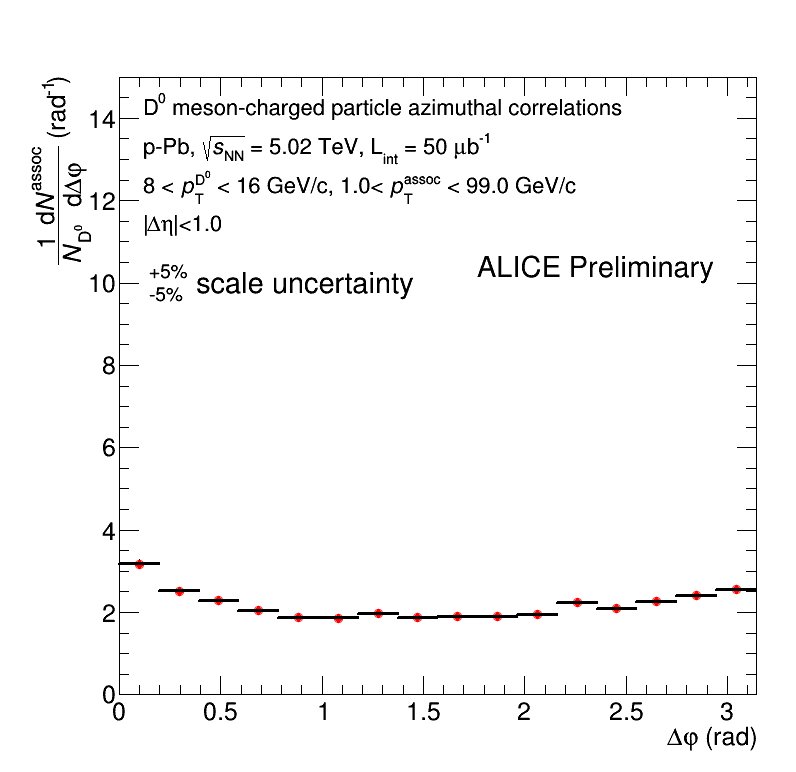
\includegraphics[width=0.32\linewidth]{figuresVsCent/Dzero/Correlations/2060/CanvaAndVariedHistopPbDzeroPt8to16assocPt1to99.png}} \\
{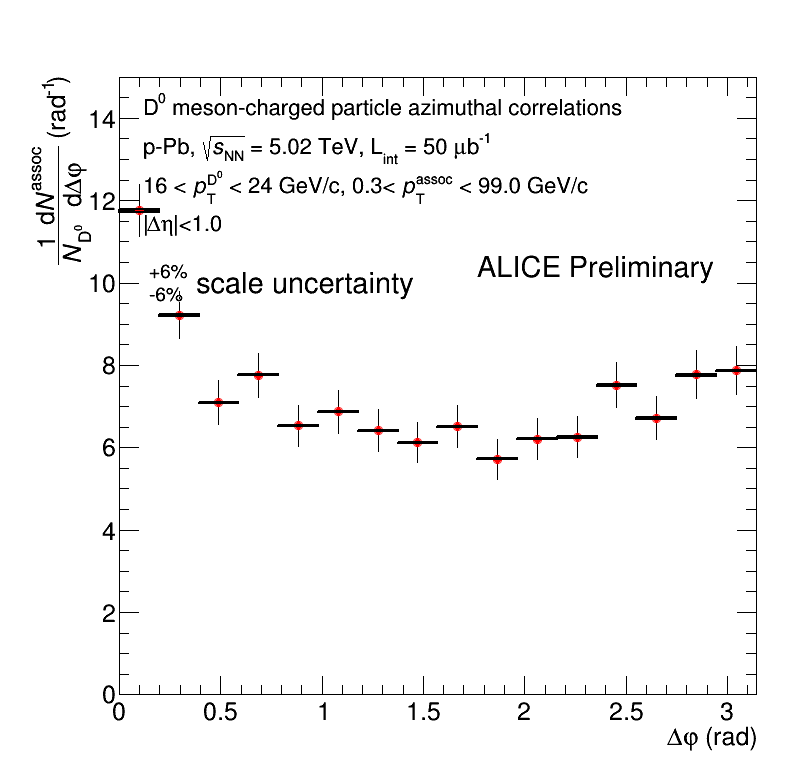
\includegraphics[width=0.32\linewidth]{figuresVsCent/Dzero/Correlations/2060/CanvaAndVariedHistopPbDzeroPt16to24assocPt03to99.png}}
{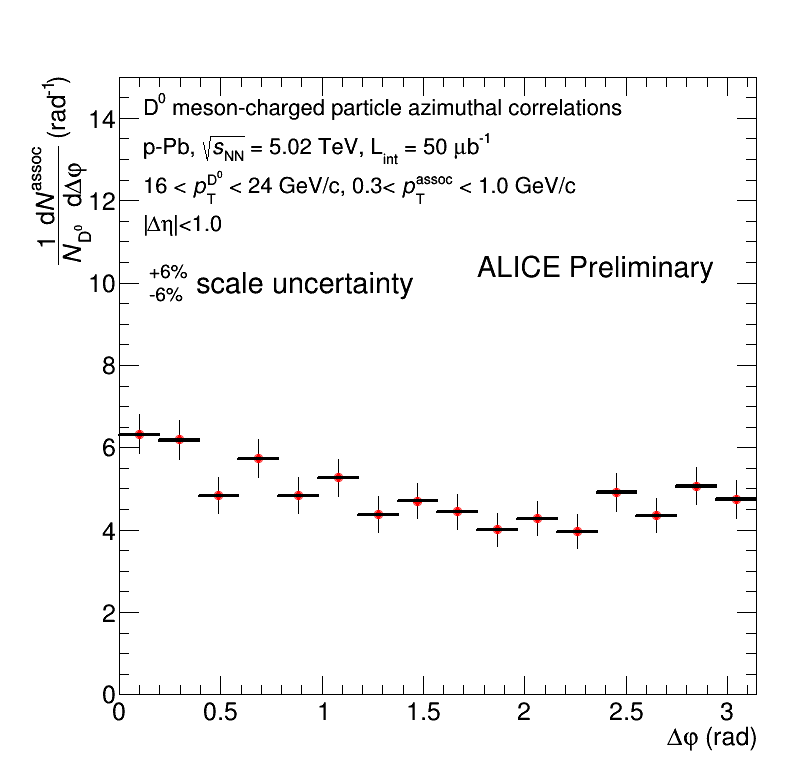
\includegraphics[width=0.32\linewidth]{figuresVsCent/Dzero/Correlations/2060/CanvaAndVariedHistopPbDzeroPt16to24assocPt03to1.png}}
{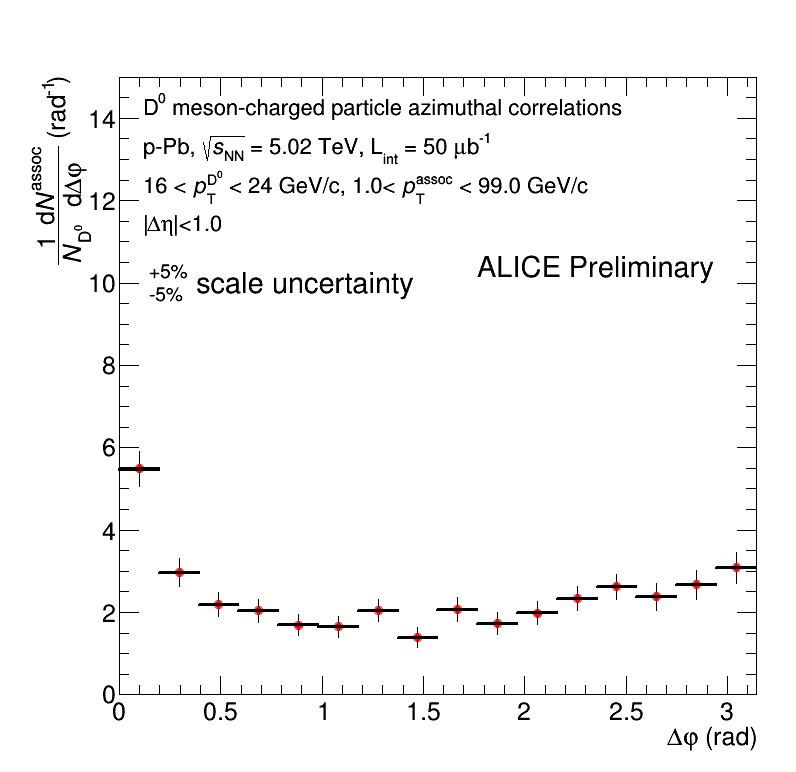
\includegraphics[width=0.32\linewidth]{figuresVsCent/Dzero/Correlations/2060/CanvaAndVariedHistopPbDzeroPt16to24assocPt1to99.png}}
 \caption{Correlation distributions for $\Dzero$ meson as trigger particle (20-60\%). Each row is a different $\pt$(D) range, each column a different $\pt$(assoc) range. The systematic uncertainties labelled in the plots are not final. Note: the L=50 $\mu$b$^-1$ is a typo of the drawing macro (it shall be 300 $\mu$b$^-1$).}
\label{fig:Dzerocorr2060}
\end{figure}

\begin{figure}
\centering
{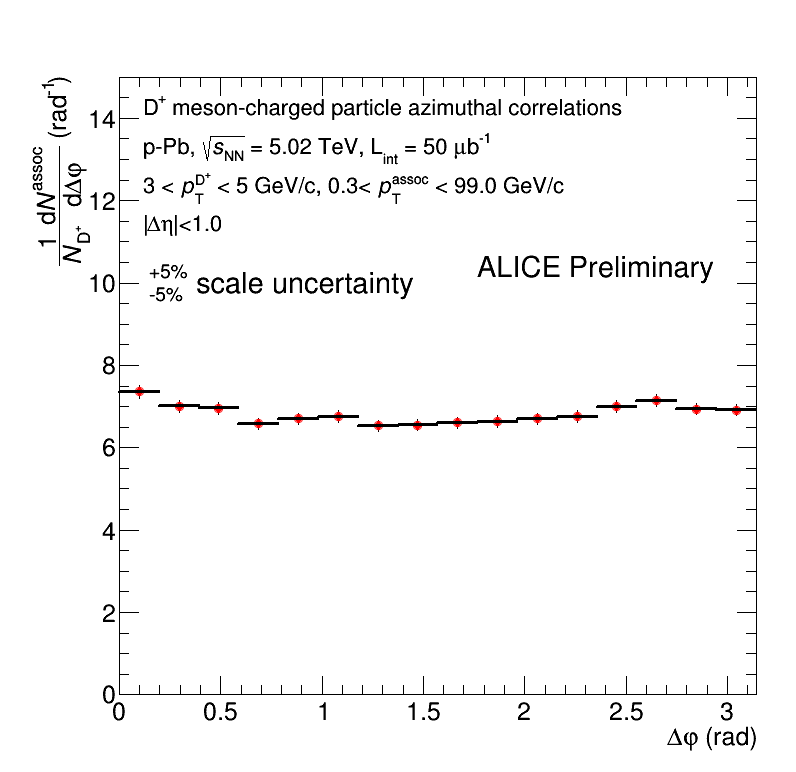
\includegraphics[width=0.32\linewidth]{figuresVsCent/Dplus/Correlations/2060/CanvaAndVariedHistopPbDplusPt3to5assocPt03to99.png}}
{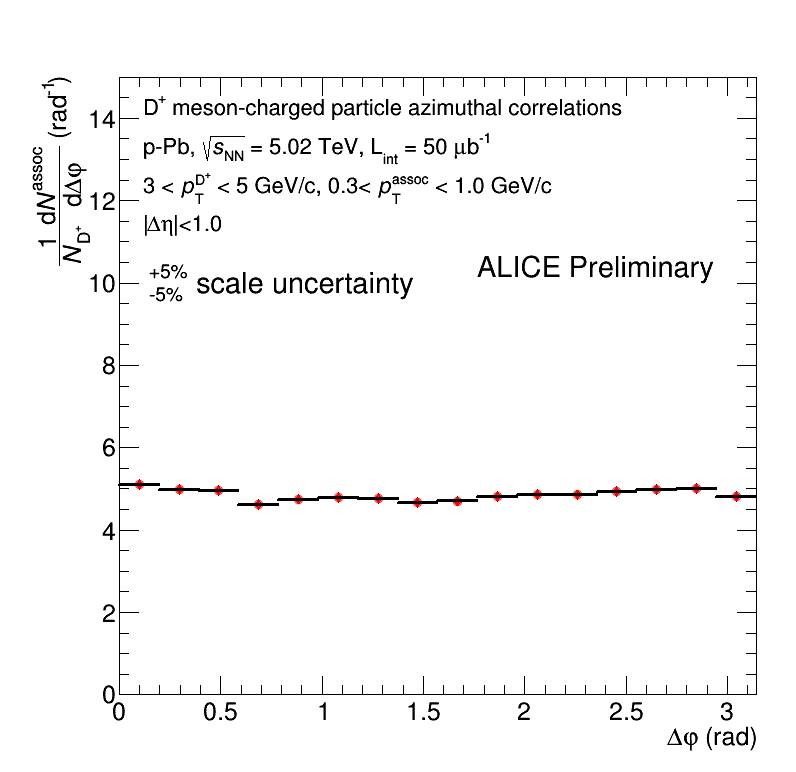
\includegraphics[width=0.32\linewidth]{figuresVsCent/Dplus/Correlations/2060/CanvaAndVariedHistopPbDplusPt3to5assocPt03to1.png}}
{\includegraphics[width=0.32\linewidth]{figuresVsCent/Dplus/Correlations/2060/CanvaAndVariedHistopPbDplusPt3to5assocPt1to99.png}} \\
{\includegraphics[width=0.32\linewidth]{figuresVsCent/Dplus/Correlations/2060/CanvaAndVariedHistopPbDplusPt5to8assocPt03to99.png}}
{\includegraphics[width=0.32\linewidth]{figuresVsCent/Dplus/Correlations/2060/CanvaAndVariedHistopPbDplusPt5to8assocPt03to1.png}}
{\includegraphics[width=0.32\linewidth]{figuresVsCent/Dplus/Correlations/2060/CanvaAndVariedHistopPbDplusPt5to8assocPt1to99.png}} \\
{\includegraphics[width=0.32\linewidth]{figuresVsCent/Dplus/Correlations/2060/CanvaAndVariedHistopPbDplusPt8to16assocPt03to99.png}}
{\includegraphics[width=0.32\linewidth]{figuresVsCent/Dplus/Correlations/2060/CanvaAndVariedHistopPbDplusPt8to16assocPt03to1.png}}
{\includegraphics[width=0.32\linewidth]{figuresVsCent/Dplus/Correlations/2060/CanvaAndVariedHistopPbDplusPt8to16assocPt1to99.png}} \\
{\includegraphics[width=0.32\linewidth]{figuresVsCent/Dplus/Correlations/2060/CanvaAndVariedHistopPbDplusPt16to24assocPt03to99.png}}
{\includegraphics[width=0.32\linewidth]{figuresVsCent/Dplus/Correlations/2060/CanvaAndVariedHistopPbDplusPt16to24assocPt03to1.png}}
{\includegraphics[width=0.32\linewidth]{figuresVsCent/Dplus/Correlations/2060/CanvaAndVariedHistopPbDplusPt16to24assocPt1to99.png}}
 \caption{Correlation distributions for $\Dplus$ meson as trigger particle (20-60\%). Each row is a different $\pt$(D) range, each column a different $\pt$(assoc) range. The systematic uncertainties labelled in the plots are not final. Note: the L=50 $\mu$b$^-1$ is a typo of the drawing macro (it shall be 300 $\mu$b$^-1$).}
\label{fig:Dpluscorr2060}
\end{figure}

\begin{figure}
\centering
{\includegraphics[width=0.32\linewidth]{figuresVsCent/Dstar/Correlations/2060/CanvaAndVariedHistopPbDstarPt3to5assocPt03to99.png}}
{\includegraphics[width=0.32\linewidth]{figuresVsCent/Dstar/Correlations/2060/CanvaAndVariedHistopPbDstarPt3to5assocPt03to1.png}}
{\includegraphics[width=0.32\linewidth]{figuresVsCent/Dstar/Correlations/2060/CanvaAndVariedHistopPbDstarPt3to5assocPt1to99.png}} \\
{\includegraphics[width=0.32\linewidth]{figuresVsCent/Dstar/Correlations/2060/CanvaAndVariedHistopPbDstarPt5to8assocPt03to99.png}}
{\includegraphics[width=0.32\linewidth]{figuresVsCent/Dstar/Correlations/2060/CanvaAndVariedHistopPbDstarPt5to8assocPt03to1.png}}
{\includegraphics[width=0.32\linewidth]{figuresVsCent/Dstar/Correlations/2060/CanvaAndVariedHistopPbDstarPt5to8assocPt1to99.png}} \\
{\includegraphics[width=0.32\linewidth]{figuresVsCent/Dstar/Correlations/2060/CanvaAndVariedHistopPbDstarPt8to16assocPt03to99.png}}
{\includegraphics[width=0.32\linewidth]{figuresVsCent/Dstar/Correlations/2060/CanvaAndVariedHistopPbDstarPt8to16assocPt03to1.png}}
{\includegraphics[width=0.32\linewidth]{figuresVsCent/Dstar/Correlations/2060/CanvaAndVariedHistopPbDstarPt8to16assocPt1to99.png}} \\
{\includegraphics[width=0.32\linewidth]{figuresVsCent/Dstar/Correlations/2060/CanvaAndVariedHistopPbDstarPt16to24assocPt03to99.png}}
{\includegraphics[width=0.32\linewidth]{figuresVsCent/Dstar/Correlations/2060/CanvaAndVariedHistopPbDstarPt16to24assocPt03to1.png}}
{\includegraphics[width=0.32\linewidth]{figuresVsCent/Dstar/Correlations/2060/CanvaAndVariedHistopPbDstarPt16to24assocPt1to99.png}}
 \caption{Correlation distributions for $\Dstar$ meson as trigger particle (20-60\%). Each row is a different $\pt$(D) range, each column a different $\pt$(assoc) range. The systematic uncertainties labelled in the plots are not final. Note: the L=50 $\mu$b$^-1$ is a typo of the drawing macro (it shall be 300 $\mu$b$^-1$).}
\label{fig:Dstarcorr2060}
\end{figure}

\begin{figure}
\centering
{\includegraphics[width=0.32\linewidth]{figuresVsCent/Dzero/Correlations/60100/CanvaAndVariedHistopPbDzeroPt3to5assocPt03to99.png}}
{\includegraphics[width=0.32\linewidth]{figuresVsCent/Dzero/Correlations/60100/CanvaAndVariedHistopPbDzeroPt3to5assocPt03to1.png}}
{\includegraphics[width=0.32\linewidth]{figuresVsCent/Dzero/Correlations/60100/CanvaAndVariedHistopPbDzeroPt3to5assocPt1to99.png}} \\
{\includegraphics[width=0.32\linewidth]{figuresVsCent/Dzero/Correlations/60100/CanvaAndVariedHistopPbDzeroPt5to8assocPt03to99.png}}
{\includegraphics[width=0.32\linewidth]{figuresVsCent/Dzero/Correlations/60100/CanvaAndVariedHistopPbDzeroPt5to8assocPt03to1.png}}
{\includegraphics[width=0.32\linewidth]{figuresVsCent/Dzero/Correlations/60100/CanvaAndVariedHistopPbDzeroPt5to8assocPt1to99.png}} \\
{\includegraphics[width=0.32\linewidth]{figuresVsCent/Dzero/Correlations/60100/CanvaAndVariedHistopPbDzeroPt8to16assocPt03to99.png}}
{\includegraphics[width=0.32\linewidth]{figuresVsCent/Dzero/Correlations/60100/CanvaAndVariedHistopPbDzeroPt8to16assocPt03to1.png}}
{\includegraphics[width=0.32\linewidth]{figuresVsCent/Dzero/Correlations/60100/CanvaAndVariedHistopPbDzeroPt8to16assocPt1to99.png}} \\
{\includegraphics[width=0.32\linewidth]{figuresVsCent/Dzero/Correlations/60100/CanvaAndVariedHistopPbDzeroPt16to24assocPt03to99.png}}
{\includegraphics[width=0.32\linewidth]{figuresVsCent/Dzero/Correlations/60100/CanvaAndVariedHistopPbDzeroPt16to24assocPt03to1.png}}
{\includegraphics[width=0.32\linewidth]{figuresVsCent/Dzero/Correlations/60100/CanvaAndVariedHistopPbDzeroPt16to24assocPt1to99.png}}
 \caption{Correlation distributions for $\Dzero$ meson as trigger particle (60-100\%). Each row is a different $\pt$(D) range, each column a different $\pt$(assoc) range. The systematic uncertainties labelled in the plots are not final. Note: the L=50 $\mu$b$^-1$ is a typo of the drawing macro (it shall be 300 $\mu$b$^-1$).}
\label{fig:Dzerocorr60100}
\end{figure}

\begin{figure}
\centering
{\includegraphics[width=0.32\linewidth]{figuresVsCent/Dplus/Correlations/60100/CanvaAndVariedHistopPbDplusPt3to5assocPt03to99.png}}
{\includegraphics[width=0.32\linewidth]{figuresVsCent/Dplus/Correlations/60100/CanvaAndVariedHistopPbDplusPt3to5assocPt03to1.png}}
{\includegraphics[width=0.32\linewidth]{figuresVsCent/Dplus/Correlations/60100/CanvaAndVariedHistopPbDplusPt3to5assocPt1to99.png}} \\
{\includegraphics[width=0.32\linewidth]{figuresVsCent/Dplus/Correlations/60100/CanvaAndVariedHistopPbDplusPt5to8assocPt03to99.png}}
{\includegraphics[width=0.32\linewidth]{figuresVsCent/Dplus/Correlations/60100/CanvaAndVariedHistopPbDplusPt5to8assocPt03to1.png}}
{\includegraphics[width=0.32\linewidth]{figuresVsCent/Dplus/Correlations/60100/CanvaAndVariedHistopPbDplusPt5to8assocPt1to99.png}} \\
{\includegraphics[width=0.32\linewidth]{figuresVsCent/Dplus/Correlations/60100/CanvaAndVariedHistopPbDplusPt8to16assocPt03to99.png}}
{\includegraphics[width=0.32\linewidth]{figuresVsCent/Dplus/Correlations/60100/CanvaAndVariedHistopPbDplusPt8to16assocPt03to1.png}}
{\includegraphics[width=0.32\linewidth]{figuresVsCent/Dplus/Correlations/60100/CanvaAndVariedHistopPbDplusPt8to16assocPt1to99.png}} \\
{\includegraphics[width=0.32\linewidth]{figuresVsCent/Dplus/Correlations/60100/CanvaAndVariedHistopPbDplusPt16to24assocPt03to99.png}}
{\includegraphics[width=0.32\linewidth]{figuresVsCent/Dplus/Correlations/60100/CanvaAndVariedHistopPbDplusPt16to24assocPt03to1.png}}
{\includegraphics[width=0.32\linewidth]{figuresVsCent/Dplus/Correlations/60100/CanvaAndVariedHistopPbDplusPt16to24assocPt1to99.png}}
 \caption{Correlation distributions for $\Dplus$ meson as trigger particle (60-100\%). Each row is a different $\pt$(D) range, each column a different $\pt$(assoc) range. The systematic uncertainties labelled in the plots are not final. Note: the L=50 $\mu$b$^-1$ is a typo of the drawing macro (it shall be 300 $\mu$b$^-1$).}
\label{fig:Dpluscorr60100}
\end{figure}

\begin{figure}
\centering
{\includegraphics[width=0.32\linewidth]{figuresVsCent/Dstar/Correlations/60100/CanvaAndVariedHistopPbDstarPt3to5assocPt03to99.png}}
{\includegraphics[width=0.32\linewidth]{figuresVsCent/Dstar/Correlations/60100/CanvaAndVariedHistopPbDstarPt3to5assocPt03to1.png}}
{\includegraphics[width=0.32\linewidth]{figuresVsCent/Dstar/Correlations/60100/CanvaAndVariedHistopPbDstarPt3to5assocPt1to99.png}} \\
{\includegraphics[width=0.32\linewidth]{figuresVsCent/Dstar/Correlations/60100/CanvaAndVariedHistopPbDstarPt5to8assocPt03to99.png}}
{\includegraphics[width=0.32\linewidth]{figuresVsCent/Dstar/Correlations/60100/CanvaAndVariedHistopPbDstarPt5to8assocPt03to1.png}}
{\includegraphics[width=0.32\linewidth]{figuresVsCent/Dstar/Correlations/60100/CanvaAndVariedHistopPbDstarPt5to8assocPt1to99.png}} \\
{\includegraphics[width=0.32\linewidth]{figuresVsCent/Dstar/Correlations/60100/CanvaAndVariedHistopPbDstarPt8to16assocPt03to99.png}}
{\includegraphics[width=0.32\linewidth]{figuresVsCent/Dstar/Correlations/60100/CanvaAndVariedHistopPbDstarPt8to16assocPt03to1.png}}
{\includegraphics[width=0.32\linewidth]{figuresVsCent/Dstar/Correlations/60100/CanvaAndVariedHistopPbDstarPt8to16assocPt1to99.png}} \\
{\includegraphics[width=0.32\linewidth]{figuresVsCent/Dstar/Correlations/60100/CanvaAndVariedHistopPbDstarPt16to24assocPt03to99.png}}
{\includegraphics[width=0.32\linewidth]{figuresVsCent/Dstar/Correlations/60100/CanvaAndVariedHistopPbDstarPt16to24assocPt03to1.png}}
{\includegraphics[width=0.32\linewidth]{figuresVsCent/Dstar/Correlations/60100/CanvaAndVariedHistopPbDstarPt16to24assocPt1to99.png}}
 \caption{Correlation distributions for $\Dstar$ meson as trigger particle (60-100\%). Each row is a different $\pt$(D) range, each column a different $\pt$(assoc) range. The systematic uncertainties labelled in the plots are not final. Note: the L=50 $\mu$b$^-1$ is a typo of the drawing macro (it shall be 300 $\mu$b$^-1$).}
\label{fig:Dstarcorr60100}
\end{figure}

\subsubsection{Average-D correlation distributions}
The average D-hadron correlation distributions are shown in Fig. \ref{fig:avgcorr020}, \ref{fig:avgcorr2060}, \ref{fig:avgcorr60100} for all the kinematic ranges and for each of the centrality classes.

\begin{figure}
\centering
{\includegraphics[width=0.32\linewidth]{figuresVsCent/Averages/020/CanvaAndVariedHistoWeightedAverageDzeroDstarDplus_pPb_Pt3to5assocPt03to99.png}}
{\includegraphics[width=0.32\linewidth]{figuresVsCent/Averages/020/CanvaAndVariedHistoWeightedAverageDzeroDstarDplus_pPb_Pt3to5assocPt03to1.png}}
{\includegraphics[width=0.32\linewidth]{figuresVsCent/Averages/020/CanvaAndVariedHistoWeightedAverageDzeroDstarDplus_pPb_Pt3to5assocPt1to99.png}} \\
{\includegraphics[width=0.32\linewidth]{figuresVsCent/Averages/020/CanvaAndVariedHistoWeightedAverageDzeroDstarDplus_pPb_Pt3to5assocPt03to99.png}}
{\includegraphics[width=0.32\linewidth]{figuresVsCent/Averages/020/CanvaAndVariedHistoWeightedAverageDzeroDstarDplus_pPb_Pt3to5assocPt03to1.png}}
{\includegraphics[width=0.32\linewidth]{figuresVsCent/Averages/020/CanvaAndVariedHistoWeightedAverageDzeroDstarDplus_pPb_Pt3to5assocPt1to99.png}} \\
{\includegraphics[width=0.32\linewidth]{figuresVsCent/Averages/020/CanvaAndVariedHistoWeightedAverageDzeroDstarDplus_pPb_Pt3to5assocPt03to99.png}}
{\includegraphics[width=0.32\linewidth]{figuresVsCent/Averages/020/CanvaAndVariedHistoWeightedAverageDzeroDstarDplus_pPb_Pt3to5assocPt03to1.png}}
{\includegraphics[width=0.32\linewidth]{figuresVsCent/Averages/020/CanvaAndVariedHistoWeightedAverageDzeroDstarDplus_pPb_Pt3to5assocPt1to99.png}} \\
{\includegraphics[width=0.32\linewidth]{figuresVsCent/Averages/020/CanvaAndVariedHistoWeightedAverageDzeroDstarDplus_pPb_Pt3to5assocPt03to99.png}}
{\includegraphics[width=0.32\linewidth]{figuresVsCent/Averages/020/CanvaAndVariedHistoWeightedAverageDzeroDstarDplus_pPb_Pt3to5assocPt03to1.png}}
{\includegraphics[width=0.32\linewidth]{figuresVsCent/Averages/020/CanvaAndVariedHistoWeightedAverageDzeroDstarDplus_pPb_Pt3to5assocPt1to99.png}}
 \caption{Average D-hadron correlation distributions in 0-20\% centrality class. Each row is a different $\pt$(D) range, each column a different $\pt$(assoc) range. The systematic uncertainties labelled in the plots are not final. Note: the L=50 $\mu$b$^-1$ is a typo of the drawing macro (it shall be 300 $\mu$b$^-1$).}
\label{fig:avgcorr020}
\end{figure}

\begin{figure}
\centering
{\includegraphics[width=0.32\linewidth]{figuresVsCent/Averages/2060/CanvaAndVariedHistoWeightedAverageDzeroDstarDplus_pPb_Pt3to5assocPt03to99.png}}
{\includegraphics[width=0.32\linewidth]{figuresVsCent/Averages/2060/CanvaAndVariedHistoWeightedAverageDzeroDstarDplus_pPb_Pt3to5assocPt03to1.png}}
{\includegraphics[width=0.32\linewidth]{figuresVsCent/Averages/2060/CanvaAndVariedHistoWeightedAverageDzeroDstarDplus_pPb_Pt3to5assocPt1to99.png}} \\
{\includegraphics[width=0.32\linewidth]{figuresVsCent/Averages/2060/CanvaAndVariedHistoWeightedAverageDzeroDstarDplus_pPb_Pt3to5assocPt03to99.png}}
{\includegraphics[width=0.32\linewidth]{figuresVsCent/Averages/2060/CanvaAndVariedHistoWeightedAverageDzeroDstarDplus_pPb_Pt3to5assocPt03to1.png}}
{\includegraphics[width=0.32\linewidth]{figuresVsCent/Averages/2060/CanvaAndVariedHistoWeightedAverageDzeroDstarDplus_pPb_Pt3to5assocPt1to99.png}} \\
{\includegraphics[width=0.32\linewidth]{figuresVsCent/Averages/2060/CanvaAndVariedHistoWeightedAverageDzeroDstarDplus_pPb_Pt3to5assocPt03to99.png}}
{\includegraphics[width=0.32\linewidth]{figuresVsCent/Averages/2060/CanvaAndVariedHistoWeightedAverageDzeroDstarDplus_pPb_Pt3to5assocPt03to1.png}}
{\includegraphics[width=0.32\linewidth]{figuresVsCent/Averages/2060/CanvaAndVariedHistoWeightedAverageDzeroDstarDplus_pPb_Pt3to5assocPt1to99.png}} \\
{\includegraphics[width=0.32\linewidth]{figuresVsCent/Averages/2060/CanvaAndVariedHistoWeightedAverageDzeroDstarDplus_pPb_Pt3to5assocPt03to99.png}}
{\includegraphics[width=0.32\linewidth]{figuresVsCent/Averages/2060/CanvaAndVariedHistoWeightedAverageDzeroDstarDplus_pPb_Pt3to5assocPt03to1.png}}
{\includegraphics[width=0.32\linewidth]{figuresVsCent/Averages/2060/CanvaAndVariedHistoWeightedAverageDzeroDstarDplus_pPb_Pt3to5assocPt1to99.png}}
 \caption{Average D-hadron correlation distributions in 20-60\% centrality class. Each row is a different $\pt$(D) range, each column a different $\pt$(assoc) range. The systematic uncertainties labelled in the plots are not final. Note: the L=50 $\mu$b$^-1$ is a typo of the drawing macro (it shall be 300 $\mu$b$^-1$).}
\label{fig:avgcorr2060}
\end{figure}

\begin{figure}
\centering
{\includegraphics[width=0.32\linewidth]{figuresVsCent/Averages/60100/CanvaAndVariedHistoWeightedAverageDzeroDstarDplus_pPb_Pt3to5assocPt03to99.png}}
{\includegraphics[width=0.32\linewidth]{figuresVsCent/Averages/60100/CanvaAndVariedHistoWeightedAverageDzeroDstarDplus_pPb_Pt3to5assocPt03to1.png}}
{\includegraphics[width=0.32\linewidth]{figuresVsCent/Averages/60100/CanvaAndVariedHistoWeightedAverageDzeroDstarDplus_pPb_Pt3to5assocPt1to99.png}} \\
{\includegraphics[width=0.32\linewidth]{figuresVsCent/Averages/60100/CanvaAndVariedHistoWeightedAverageDzeroDstarDplus_pPb_Pt3to5assocPt03to99.png}}
{\includegraphics[width=0.32\linewidth]{figuresVsCent/Averages/60100/CanvaAndVariedHistoWeightedAverageDzeroDstarDplus_pPb_Pt3to5assocPt03to1.png}}
{\includegraphics[width=0.32\linewidth]{figuresVsCent/Averages/60100/CanvaAndVariedHistoWeightedAverageDzeroDstarDplus_pPb_Pt3to5assocPt1to99.png}} \\
{\includegraphics[width=0.32\linewidth]{figuresVsCent/Averages/60100/CanvaAndVariedHistoWeightedAverageDzeroDstarDplus_pPb_Pt3to5assocPt03to99.png}}
{\includegraphics[width=0.32\linewidth]{figuresVsCent/Averages/60100/CanvaAndVariedHistoWeightedAverageDzeroDstarDplus_pPb_Pt3to5assocPt03to1.png}}
{\includegraphics[width=0.32\linewidth]{figuresVsCent/Averages/60100/CanvaAndVariedHistoWeightedAverageDzeroDstarDplus_pPb_Pt3to5assocPt1to99.png}} \\
{\includegraphics[width=0.32\linewidth]{figuresVsCent/Averages/60100/CanvaAndVariedHistoWeightedAverageDzeroDstarDplus_pPb_Pt3to5assocPt03to99.png}}
{\includegraphics[width=0.32\linewidth]{figuresVsCent/Averages/60100/CanvaAndVariedHistoWeightedAverageDzeroDstarDplus_pPb_Pt3to5assocPt03to1.png}}
{\includegraphics[width=0.32\linewidth]{figuresVsCent/Averages/60100/CanvaAndVariedHistoWeightedAverageDzeroDstarDplus_pPb_Pt3to5assocPt1to99.png}}
 \caption{Average D-hadron correlation distributions in 60-100\% centrality class. Each row is a different $\pt$(D) range, each column a different $\pt$(assoc) range. The systematic uncertainties labelled in the plots are not final. Note: the L=50 $\mu$b$^-1$ is a typo of the drawing macro (it shall be 300 $\mu$b$^-1$).}
\label{fig:avgcorr60100}
\end{figure}
\clearpage

\subsubsection{Observables from fit to correlation distributions}
The outcome of the fits to the above correlation distributions are shown in Fig. \ref{fig:fit020}, \ref{fig:fit2060}, \ref{fig:fit60100}, for the three centrality ranges.

\begin{figure}
\centering
{\includegraphics[width=0.8\linewidth]{figuresVsCent/Averages/020/cFitting_0_pthad03to99.png}}
{\includegraphics[width=0.8\linewidth]{figuresVsCent/Averages/020/cFitting_0_pthad03to1.png}}
{\includegraphics[width=0.8\linewidth]{figuresVsCent/Averages/020/cFitting_0_pthad1to99.png}}
 \caption{Outcome of fit to correlation distributions in 0-20\% centrality class. Each sub-figure shows the 4 $\pt$(D) ranges of a given $\pt$(assoc) range.}
\label{fig:fit020}
\end{figure}

\begin{figure}
\centering
{\includegraphics[width=0.8\linewidth]{figuresVsCent/Averages/2060/cFitting_0_pthad03to99.png}}
{\includegraphics[width=0.8\linewidth]{figuresVsCent/Averages/2060/cFitting_0_pthad03to1.png}}
{\includegraphics[width=0.8\linewidth]{figuresVsCent/Averages/2060/cFitting_0_pthad1to99.png}}
 \caption{Outcome of fit to correlation distributions in 20-60\% centrality class. Each sub-figure shows the 4 $\pt$(D) ranges of a given $\pt$(assoc) range.}
\label{fig:fit2060}
\end{figure}

\begin{figure}
\centering
{\includegraphics[width=0.8\linewidth]{figuresVsCent/Averages/60100/cFitting_0_pthad03to99.png}}
{\includegraphics[width=0.8\linewidth]{figuresVsCent/Averages/60100/cFitting_0_pthad03to1.png}}
{\includegraphics[width=0.8\linewidth]{figuresVsCent/Averages/60100/cFitting_0_pthad1to99.png}}
 \caption{Outcome of fit to correlation distributions in 60-100\% centrality class. Each sub-figure shows the 4 $\pt$(D) ranges of a given $\pt$(assoc) range.}
\label{fig:fit60100}
\end{figure}

\clearpage
In Fig. \ref{fig:obs020}, \ref{fig:obs2060}, \ref{fig:obs60100} the quantitative observables (i.e. near-side and away-side yields and widths) extracted from the fit are presented.

\begin{figure}
\centering
{\includegraphics[width=0.32\linewidth]{figuresVsCent/Averages/020/CanvasFinalTrendNSYield_pthad03to99.png}}
{\includegraphics[width=0.32\linewidth]{figuresVsCent/Averages/020/CanvasFinalTrendNSYield_pthad03to1.png}}
{\includegraphics[width=0.32\linewidth]{figuresVsCent/Averages/020/CanvasFinalTrendNSYield_pthad1to99.png}} \\
{\includegraphics[width=0.32\linewidth]{figuresVsCent/Averages/020/CanvasFinalTrendNSSigma_pthad03to99.png}}
{\includegraphics[width=0.32\linewidth]{figuresVsCent/Averages/020/CanvasFinalTrendNSSigma_pthad03to1.png}}
{\includegraphics[width=0.32\linewidth]{figuresVsCent/Averages/020/CanvasFinalTrendNSSigma_pthad1to99.png}} \\
{\includegraphics[width=0.32\linewidth]{figuresVsCent/Averages/020/CanvasFinalTrendASYield_pthad03to99.png}}
{\includegraphics[width=0.32\linewidth]{figuresVsCent/Averages/020/CanvasFinalTrendASYield_pthad03to1.png}}
{\includegraphics[width=0.32\linewidth]{figuresVsCent/Averages/020/CanvasFinalTrendASYield_pthad1to99.png}} \\
{\includegraphics[width=0.32\linewidth]{figuresVsCent/Averages/020/CanvasFinalTrendASSigma_pthad03to99.png}}
{\includegraphics[width=0.32\linewidth]{figuresVsCent/Averages/020/CanvasFinalTrendASSigma_pthad03to1.png}}
{\includegraphics[width=0.32\linewidth]{figuresVsCent/Averages/020/CanvasFinalTrendASSigma_pthad1to99.png}} \\
 \caption{Near-side yield (rows 1-3) and width (4-6) and away-side yield (7-9) and width (10-12), for 0-20\%. Each row represents a $\pt$(assoc) range, and each panel shows the $\pt$(D) trend of the observable for a given $\pt$(assoc) range. }
\label{fig:obs020}
\end{figure}

\begin{figure}
\centering
{\includegraphics[width=0.32\linewidth]{figuresVsCent/Averages/2060/CanvasFinalTrendNSYield_pthad03to99.png}}
{\includegraphics[width=0.32\linewidth]{figuresVsCent/Averages/2060/CanvasFinalTrendNSYield_pthad03to1.png}}
{\includegraphics[width=0.32\linewidth]{figuresVsCent/Averages/2060/CanvasFinalTrendNSYield_pthad1to99.png}} \\
{\includegraphics[width=0.32\linewidth]{figuresVsCent/Averages/2060/CanvasFinalTrendNSSigma_pthad03to99.png}}
{\includegraphics[width=0.32\linewidth]{figuresVsCent/Averages/2060/CanvasFinalTrendNSSigma_pthad03to1.png}}
{\includegraphics[width=0.32\linewidth]{figuresVsCent/Averages/2060/CanvasFinalTrendNSSigma_pthad1to99.png}} \\
{\includegraphics[width=0.32\linewidth]{figuresVsCent/Averages/2060/CanvasFinalTrendASYield_pthad03to99.png}}
{\includegraphics[width=0.32\linewidth]{figuresVsCent/Averages/2060/CanvasFinalTrendASYield_pthad03to1.png}}
{\includegraphics[width=0.32\linewidth]{figuresVsCent/Averages/2060/CanvasFinalTrendASYield_pthad1to99.png}} \\
{\includegraphics[width=0.32\linewidth]{figuresVsCent/Averages/2060/CanvasFinalTrendASSigma_pthad03to99.png}}
{\includegraphics[width=0.32\linewidth]{figuresVsCent/Averages/2060/CanvasFinalTrendASSigma_pthad03to1.png}}
{\includegraphics[width=0.32\linewidth]{figuresVsCent/Averages/2060/CanvasFinalTrendASSigma_pthad1to99.png}} \\
 \caption{Near-side yield (rows 1-3) and width (4-6) and away-side yield (7-9) and width (10-12), for 20-60\%. Each row represents a $\pt$(assoc) range, and each panel shows the $\pt$(D) trend of the observable for a given $\pt$(assoc) range.}
\label{fig:obs2060}
\end{figure}

\begin{figure}
\centering
{\includegraphics[width=0.32\linewidth]{figuresVsCent/Averages/60100/CanvasFinalTrendNSYield_pthad03to99.png}}
{\includegraphics[width=0.32\linewidth]{figuresVsCent/Averages/60100/CanvasFinalTrendNSYield_pthad03to1.png}}
{\includegraphics[width=0.32\linewidth]{figuresVsCent/Averages/60100/CanvasFinalTrendNSYield_pthad1to99.png}} \\
{\includegraphics[width=0.32\linewidth]{figuresVsCent/Averages/60100/CanvasFinalTrendNSSigma_pthad03to99.png}}
{\includegraphics[width=0.32\linewidth]{figuresVsCent/Averages/60100/CanvasFinalTrendNSSigma_pthad03to1.png}}
{\includegraphics[width=0.32\linewidth]{figuresVsCent/Averages/60100/CanvasFinalTrendNSSigma_pthad1to99.png}} \\
{\includegraphics[width=0.32\linewidth]{figuresVsCent/Averages/60100/CanvasFinalTrendASYield_pthad03to99.png}}
{\includegraphics[width=0.32\linewidth]{figuresVsCent/Averages/60100/CanvasFinalTrendASYield_pthad03to1.png}}
{\includegraphics[width=0.32\linewidth]{figuresVsCent/Averages/60100/CanvasFinalTrendASYield_pthad1to99.png}} \\
{\includegraphics[width=0.32\linewidth]{figuresVsCent/Averages/60100/CanvasFinalTrendASSigma_pthad03to99.png}}
{\includegraphics[width=0.32\linewidth]{figuresVsCent/Averages/60100/CanvasFinalTrendASSigma_pthad03to1.png}}
{\includegraphics[width=0.32\linewidth]{figuresVsCent/Averages/60100/CanvasFinalTrendASSigma_pthad1to99.png}} \\
 \caption{Near-side yield (rows 1-3) and width (4-6) and away-side yield (7-9) and width (10-12), for 60-100\%. Each row represents a $\pt$(assoc) range, and each panel shows the $\pt$(D) trend of the observable for a given $\pt$(assoc) range.}
\label{fig:obs60100}
\end{figure}

\clearpage
The systematic uncertainties on the fit observables, including those related to the variation of the transverse region for the baseline evaluation, the possible presence of a $v_2$ modulation, and the $\Delta\varphi$ scaling uncertainty (for the yields only), are shown in Fig. \ref{fig:syst020}, \ref{fig:syst2060}, \ref{fig:syst60100}.

\begin{figure}
\centering
{\includegraphics[width=0.32\linewidth]{figuresVsCent/Averages/020/TotalSystematicSourcesNSYield_pthad03to99.png}}
{\includegraphics[width=0.32\linewidth]{figuresVsCent/Averages/020/TotalSystematicSourcesNSYield_pthad03to1.png}}
{\includegraphics[width=0.32\linewidth]{figuresVsCent/Averages/020/TotalSystematicSourcesNSYield_pthad1to99.png}} \\
{\includegraphics[width=0.32\linewidth]{figuresVsCent/Averages/020/TotalSystematicSourcesNSSigma_pthad03to99.png}}
{\includegraphics[width=0.32\linewidth]{figuresVsCent/Averages/020/TotalSystematicSourcesNSSigma_pthad03to1.png}}
{\includegraphics[width=0.32\linewidth]{figuresVsCent/Averages/020/TotalSystematicSourcesNSSigma_pthad1to99.png}} \\
{\includegraphics[width=0.32\linewidth]{figuresVsCent/Averages/020/TotalSystematicSourcesASYield_pthad03to99.png}}
{\includegraphics[width=0.32\linewidth]{figuresVsCent/Averages/020/TotalSystematicSourcesASYield_pthad03to1.png}}
{\includegraphics[width=0.32\linewidth]{figuresVsCent/Averages/020/TotalSystematicSourcesASYield_pthad1to99.png}} \\
{\includegraphics[width=0.32\linewidth]{figuresVsCent/Averages/020/TotalSystematicSourcesASSigma_pthad03to99.png}}
{\includegraphics[width=0.32\linewidth]{figuresVsCent/Averages/020/TotalSystematicSourcesASSigma_pthad03to1.png}}
{\includegraphics[width=0.32\linewidth]{figuresVsCent/Averages/020/TotalSystematicSourcesASSigma_pthad1to99.png}} \\
 \caption{Near-side yield (rows 1-3) and width (4-6) and away-side yield (7-9) and width (10-12), for 0-20\%. Each row represents a $\pt$(assoc) range, and each panel shows the $\pt$(D) trend of the observable for a given $\pt$(assoc) range.}
\label{fig:syst020}
\end{figure}

\begin{figure}
\centering
{\includegraphics[width=0.32\linewidth]{figuresVsCent/Averages/2060/TotalSystematicSourcesNSYield_pthad03to99.png}}
{\includegraphics[width=0.32\linewidth]{figuresVsCent/Averages/2060/TotalSystematicSourcesNSYield_pthad03to1.png}}
{\includegraphics[width=0.32\linewidth]{figuresVsCent/Averages/2060/TotalSystematicSourcesNSYield_pthad1to99.png}} \\
{\includegraphics[width=0.32\linewidth]{figuresVsCent/Averages/2060/TotalSystematicSourcesNSSigma_pthad03to99.png}}
{\includegraphics[width=0.32\linewidth]{figuresVsCent/Averages/2060/TotalSystematicSourcesNSSigma_pthad03to1.png}}
{\includegraphics[width=0.32\linewidth]{figuresVsCent/Averages/2060/TotalSystematicSourcesNSSigma_pthad1to99.png}} \\
{\includegraphics[width=0.32\linewidth]{figuresVsCent/Averages/2060/TotalSystematicSourcesASYield_pthad03to99.png}}
{\includegraphics[width=0.32\linewidth]{figuresVsCent/Averages/2060/TotalSystematicSourcesASYield_pthad03to1.png}}
{\includegraphics[width=0.32\linewidth]{figuresVsCent/Averages/2060/TotalSystematicSourcesASYield_pthad1to99.png}} \\
{\includegraphics[width=0.32\linewidth]{figuresVsCent/Averages/2060/TotalSystematicSourcesASSigma_pthad03to99.png}}
{\includegraphics[width=0.32\linewidth]{figuresVsCent/Averages/2060/TotalSystematicSourcesASSigma_pthad03to1.png}}
{\includegraphics[width=0.32\linewidth]{figuresVsCent/Averages/2060/TotalSystematicSourcesASSigma_pthad1to99.png}} \\
 \caption{Near-side yield (rows 1-3) and width (4-6) and away-side yield (7-9) and width (10-12), for 20-60\%. Each row represents a $\pt$(assoc) range, and each panel shows the $\pt$(D) trend of the observable for a given $\pt$(assoc) range.}
\label{fig:syst2060}
\end{figure}

\begin{figure}
\centering
{\includegraphics[width=0.32\linewidth]{figuresVsCent/Averages/60100/TotalSystematicSourcesNSYield_pthad03to99.png}}
{\includegraphics[width=0.32\linewidth]{figuresVsCent/Averages/60100/TotalSystematicSourcesNSYield_pthad03to1.png}}
{\includegraphics[width=0.32\linewidth]{figuresVsCent/Averages/60100/TotalSystematicSourcesNSYield_pthad1to99.png}} \\
{\includegraphics[width=0.32\linewidth]{figuresVsCent/Averages/60100/TotalSystematicSourcesNSSigma_pthad03to99.png}}
{\includegraphics[width=0.32\linewidth]{figuresVsCent/Averages/60100/TotalSystematicSourcesNSSigma_pthad03to1.png}}
{\includegraphics[width=0.32\linewidth]{figuresVsCent/Averages/60100/TotalSystematicSourcesNSSigma_pthad1to99.png}} \\
{\includegraphics[width=0.32\linewidth]{figuresVsCent/Averages/60100/TotalSystematicSourcesASYield_pthad03to99.png}}
{\includegraphics[width=0.32\linewidth]{figuresVsCent/Averages/60100/TotalSystematicSourcesASYield_pthad03to1.png}}
{\includegraphics[width=0.32\linewidth]{figuresVsCent/Averages/60100/TotalSystematicSourcesASYield_pthad1to99.png}} \\
{\includegraphics[width=0.32\linewidth]{figuresVsCent/Averages/60100/TotalSystematicSourcesASSigma_pthad03to99.png}}
{\includegraphics[width=0.32\linewidth]{figuresVsCent/Averages/60100/TotalSystematicSourcesASSigma_pthad03to1.png}}
{\includegraphics[width=0.32\linewidth]{figuresVsCent/Averages/60100/TotalSystematicSourcesASSigma_pthad1to99.png}} \\
 \caption{Near-side yield (rows 1-3) and width (4-6) and away-side yield (7-9) and width (10-12), for 60-100\%. Each row represents a $\pt$(assoc) range, and each panel shows the $\pt$(D) trend of the observable for a given $\pt$(assoc) range.}
\label{fig:syst60100}
\end{figure}

\clearpage
In particular, the breakdown of the uncertainties coming from the alternate fits done with different transverse region definition (as well as from the alternate fits by moving the baseline value from its default value) are shown in Fig. \ref{fig:basel020}, \ref{fig:basel2060}, \ref{fig:basel60100}.

\begin{figure}
\centering
{\includegraphics[width=0.32\linewidth]{figuresVsCent/Averages/020/BaselineSystematicSourcesNSYield_pthad03to99.png}}
{\includegraphics[width=0.32\linewidth]{figuresVsCent/Averages/020/BaselineSystematicSourcesNSYield_pthad03to1.png}}
{\includegraphics[width=0.32\linewidth]{figuresVsCent/Averages/020/BaselineSystematicSourcesNSYield_pthad1to99.png}} \\
{\includegraphics[width=0.32\linewidth]{figuresVsCent/Averages/020/BaselineSystematicSourcesNSSigma_pthad03to99.png}}
{\includegraphics[width=0.32\linewidth]{figuresVsCent/Averages/020/BaselineSystematicSourcesNSSigma_pthad03to1.png}}
{\includegraphics[width=0.32\linewidth]{figuresVsCent/Averages/020/BaselineSystematicSourcesNSSigma_pthad1to99.png}} \\
{\includegraphics[width=0.32\linewidth]{figuresVsCent/Averages/020/BaselineSystematicSourcesASYield_pthad03to99.png}}
{\includegraphics[width=0.32\linewidth]{figuresVsCent/Averages/020/BaselineSystematicSourcesASYield_pthad03to1.png}}
{\includegraphics[width=0.32\linewidth]{figuresVsCent/Averages/020/BaselineSystematicSourcesASYield_pthad1to99.png}} \\
{\includegraphics[width=0.32\linewidth]{figuresVsCent/Averages/020/BaselineSystematicSourcesASSigma_pthad03to99.png}}
{\includegraphics[width=0.32\linewidth]{figuresVsCent/Averages/020/BaselineSystematicSourcesASSigma_pthad03to1.png}}
{\includegraphics[width=0.32\linewidth]{figuresVsCent/Averages/020/BaselineSystematicSourcesASSigma_pthad1to99.png}} \\
 \caption{Near-side yield (rows 1-3) and width (4-6) and away-side yield (7-9) and width (10-12), for 0-20\%. Each row represents a $\pt$(assoc) range, and each panel shows the $\pt$(D) trend of the observable for a given $\pt$(assoc) range.}
\label{fig:basel020}
\end{figure}

\begin{figure}
\centering
{\includegraphics[width=0.32\linewidth]{figuresVsCent/Averages/2060/BaselineSystematicSourcesNSYield_pthad03to99.png}}
{\includegraphics[width=0.32\linewidth]{figuresVsCent/Averages/2060/BaselineSystematicSourcesNSYield_pthad03to1.png}}
{\includegraphics[width=0.32\linewidth]{figuresVsCent/Averages/2060/BaselineSystematicSourcesNSYield_pthad1to99.png}} \\
{\includegraphics[width=0.32\linewidth]{figuresVsCent/Averages/2060/BaselineSystematicSourcesNSSigma_pthad03to99.png}}
{\includegraphics[width=0.32\linewidth]{figuresVsCent/Averages/2060/BaselineSystematicSourcesNSSigma_pthad03to1.png}}
{\includegraphics[width=0.32\linewidth]{figuresVsCent/Averages/2060/BaselineSystematicSourcesNSSigma_pthad1to99.png}} \\
{\includegraphics[width=0.32\linewidth]{figuresVsCent/Averages/2060/BaselineSystematicSourcesASYield_pthad03to99.png}}
{\includegraphics[width=0.32\linewidth]{figuresVsCent/Averages/2060/BaselineSystematicSourcesASYield_pthad03to1.png}}
{\includegraphics[width=0.32\linewidth]{figuresVsCent/Averages/2060/BaselineSystematicSourcesASYield_pthad1to99.png}} \\
{\includegraphics[width=0.32\linewidth]{figuresVsCent/Averages/2060/BaselineSystematicSourcesASSigma_pthad03to99.png}}
{\includegraphics[width=0.32\linewidth]{figuresVsCent/Averages/2060/BaselineSystematicSourcesASSigma_pthad03to1.png}}
{\includegraphics[width=0.32\linewidth]{figuresVsCent/Averages/2060/BaselineSystematicSourcesASSigma_pthad1to99.png}} \\
 \caption{Near-side yield (rows 1-3) and width (4-6) and away-side yield (7-9) and width (10-12), for 20-60\%. Each row represents a $\pt$(assoc) range, and each panel shows the $\pt$(D) trend of the observable for a given $\pt$(assoc) range.}
\label{fig:basel2060}
\end{figure}

\begin{figure}
\centering
{\includegraphics[width=0.32\linewidth]{figuresVsCent/Averages/60100/BaselineSystematicSourcesNSYield_pthad03to99.png}}
{\includegraphics[width=0.32\linewidth]{figuresVsCent/Averages/60100/BaselineSystematicSourcesNSYield_pthad03to1.png}}
{\includegraphics[width=0.32\linewidth]{figuresVsCent/Averages/60100/BaselineSystematicSourcesNSYield_pthad1to99.png}} \\
{\includegraphics[width=0.32\linewidth]{figuresVsCent/Averages/60100/BaselineSystematicSourcesNSSigma_pthad03to99.png}}
{\includegraphics[width=0.32\linewidth]{figuresVsCent/Averages/60100/BaselineSystematicSourcesNSSigma_pthad03to1.png}}
{\includegraphics[width=0.32\linewidth]{figuresVsCent/Averages/60100/BaselineSystematicSourcesNSSigma_pthad1to99.png}} \\
{\includegraphics[width=0.32\linewidth]{figuresVsCent/Averages/60100/BaselineSystematicSourcesASYield_pthad03to99.png}}
{\includegraphics[width=0.32\linewidth]{figuresVsCent/Averages/60100/BaselineSystematicSourcesASYield_pthad03to1.png}}
{\includegraphics[width=0.32\linewidth]{figuresVsCent/Averages/60100/BaselineSystematicSourcesASYield_pthad1to99.png}} \\
{\includegraphics[width=0.32\linewidth]{figuresVsCent/Averages/60100/BaselineSystematicSourcesASSigma_pthad03to99.png}}
{\includegraphics[width=0.32\linewidth]{figuresVsCent/Averages/60100/BaselineSystematicSourcesASSigma_pthad03to1.png}}
{\includegraphics[width=0.32\linewidth]{figuresVsCent/Averages/60100/BaselineSystematicSourcesASSigma_pthad1to99.png}} \\
 \caption{Near-side yield (rows 1-3) and width (4-6) and away-side yield (7-9) and width (10-12), for 60-100\%. Each row represents a $\pt$(assoc) range, and each panel shows the $\pt$(D) trend of the observable for a given $\pt$(assoc) range.}
\label{fig:basel60100}
\end{figure}

\subsubsection{Plots proposed for preliminaries}
In the following, the two figures for which an approval as preliminary is requested are presented.

The first, Fig. \ref{fig:prel1}, is a comparison of the correlation distributions, after the baseline subtraction, among the three centrality classes (showing also the 0-100\% results, i.e. the previously approved preliminary results). Each panel represents a different kinematic range. In all the three centrality classes, the correlation distributions show very similar shapes of the correlation peaks, and a consistent $\pt$ evolution. Most probably, the last column will be cropped, due to the too large statistical uncertainty on the 16-24 GeV/$c$ correlation distributions.

\begin{landscape}
\begin{figure}
\centering
{\includegraphics[width=0.9\linewidth]{figuresVsCent/Averages/Trends/plotComparison_WeightedAverage_pp_pPb_UniqueCanvas_Style1_FinalQM.png}}
 \caption{Comparison of baseline-subtracted correlation distributions in the different centrality classes. Each color is a different centrality class, as described in the legend. The error bars represent the statistical uncertainty, the empty boxes represent the overall systematic uncertainties, the shaded boxed represent the $v_2$ related uncertainties.}
\label{fig:prel1}
\end{figure}
\end{landscape}

The second, Fig. \ref{fig:prel2}, is a comparison of the near-side fit observables (yields and width) among the three centrality classes, also here showing the 0-100\% results as well, i.e. the previously approved preliminary results. Within the current uncertainties, no clear modifications of the near-side peak properties appear for the different centrality classes (nor w.r.t. the 0-100\% results). The same increasing trend with $\pt$(D) is observed, due to the increased energy of the originally parton which results in more production of fragmentation tracks, as a similar slight decrease of the peak sigma when going to higher $\pt$(D) is also observed, due to the stronger collimation of the fragmentation tracks of the charm quark. The small value of the yield in the 3-5 GeV/$c$ range in 60-100\% (especially for the higher $\pt$(assoc) range) is most probably not a physical feature, but comes from an unlucky positioning of the points at $\Delta\varphi \approx 0$ of the azimuthal correlation (mainly due to fluctuations), especially for the first point, as it can be seen from the previous figure (green points).

\begin{landscape}
\begin{figure}
\centering
{\includegraphics[width=0.95\linewidth]{figuresVsCent/Averages/Trends/ComparePPbVsCentFitResults_FinalQM.png}}
 \caption{Comparison of near-side observables in the different centrality classes. Each color is a different centrality class, as described in the legend. The error bars represent the statistical uncertainty, the empty boxes represent the overall systematic uncertainties, the shaded boxed represent the $v_2$ related uncertainties.}
\label{fig:prel2}
\end{figure}
\end{landscape}

For completeness, the comparison of the away-side fit observables are also shown in Fig. \ref{fig:prel3}. Anyway, due to the too large uncertainties, especially those related to the fitting procedure, we will most probably not request an approval for this figure. Indeed, some of the fits even fail in reproducing the away-side peak, while this doesn't happen for the near-side peak region. On top of the uncertainties, an increase of the yields with $\pt$(D), though probably slightly milder than for the near-side, can be observed, as well as a very similar sligthly decreasing trend for the away-side width - though the values are approximately twofold w.r.t. the near-side width.

\begin{landscape}
\begin{figure}
\centering
{\includegraphics[width=0.95\linewidth]{figuresVsCent/Averages/Trends/ComparePPbVsCentFitResults_AwaySide_FinalQM.png}}
 \caption{Comparison of away-side observables in the different centrality classes. Each color is a different centrality class, as described in the legend. The error bars represent the statistical uncertainty, the empty boxes represent the overall systematic uncertainties, the shaded boxed represent the $v_2$ related uncertainties.}
\label{fig:prel3}
\end{figure}
 \end{landscape} 
